%文档整合 Chaoming_Gu 2018.4.18
\documentclass{beamer}
\usepackage{ctex}
\usepackage{graphicx,hyperref,url}
\usepackage{amsmath,amsfonts,amssymb,bm} 
\newtheorem{proposition}[theorem]{Proposition}
\renewcommand{\proofname}{标准布朗运动的数学性质}
\usepackage{booktabs}
\usepackage{ccicons} %%[scale=2]
\usepackage{listings}
\usepackage{tikz}
\usepackage[linesnumbered,ruled]{algorithm2e}
\usepackage{algorithmicx}
\usepackage{algpseudocode}
\usepackage{float}
\usepackage{xspace}
\usepackage{appendixnumberbeamer}
\usepackage{fontspec}
\usecolortheme{beaver}
\newcommand{\tnewroman}{\fontspec{Helvetica}}

\begin{document}

\begin{frame}
	\title{觅食算法}
	\author{李昱辰\ 张恒\ 时侠圣\ 李崇慧\ 刘子旋\ 潘镇涛\ 朱春林\ 谷超明}
	\date{2018年4月19日}
	\titlepage
\end{frame}

\begin{frame}{目录}
\tableofcontents
\end{frame}


%%%%%%%%_1_
%\usepackage[BoldFont,SlantFont,CJKchecksingle]{xeCJK}
%\setCJKmainfont[BoldFont=SimHei,SlantedFont=KaiTi]{SimSun}
%\setCJKsansfont[BoldFont=SimHei,SlantedFont=KaiTi]{SimSun}
%\setCJKmonofont[ItalicFont={Adobe Fangsong Std}]{SimSun}
%\setCJKfamilyfont{zhsong}{SimSun}
%\setCJKfamilyfont{zhhei}{SimHei}
%\setCJKfamilyfont{zhkai}{KaiTi}
%\setCJKfamilyfont{zhfs}{FangSong}

%\usepackage{pgfplots}
%\usepgfplotslibrary{dateplot}



%\newcommand{\themename}{\textbf{\textsc{metropolis}}\xspace}
\section{觅食算法之布朗运动}
\title{觅食算法之布朗运动}
\frame{
	\centerline{\textbf{\Huge{觅食算法之布朗运动}}}
}
%\subtitle{A modern beamer theme}
%\date{\today}

%\author{李崇慧}
%\institute{浙江大学人文学院}
%\titlegraphic{\hfill\includegraphics[height=1.5cm]{logo.pdf}}


	
%	\maketitle
	
	
	\frame{\frametitle{随机过程与布朗运动}
		\parindent=19pt	
		\renewcommand{\raggedright}{\leftskip=0pt \rightskip=0pt plus 0cm}
		\raggedright	
		我们周边充满了各种各样的数据,所谓大数据时代,这些数据最基本的特点就是含有巨量的噪音,而随机过程就是尝试从这些噪音里提取出信息。
		
		随机过程描述的是一个量随时间可能的变化,在这个过程里,每一个时刻变化的方向都是不确定的,或者说随机过程就是由一系列随机变量组成,每一个时刻系统的状态都由一个随机变量表述,而整个过程则构成态空间的一个轨迹(随机过程的实现)。
		
	}
	
	\frame{\frametitle{布朗运动的简史}
		\parindent=19pt	
		\renewcommand{\raggedright}{\leftskip=0pt \rightskip=0pt plus 0cm}
		\raggedright	
		最初由英国生物学家布朗(Brown)于1827年提出这种物理现象。1905年爱因斯坦首次对这一现象的物理规律给出数学描述。1918年维纳(Wiener)运用数学理论严格描述这种无规则运动。并用随机过程理论和概率理论建立了数学模型。因此又称为维纳过程。是具有连续时间参数和连续状态空间的一类随机过程。
		
		自1860年以来,许多科学家都在研究此种现象,后来发现布朗运动有下列的主要特性:
		\begin{itemize}
			\item 粒子的运动由平移及转移所构成,显得非常没规则而且其轨迹几乎是处处没有切线。
			\item 粒子之移动显然互不相关,甚至于当粒子互相接近至比其直径小的距离时也是如此。
			\item 粒子的成分及密度对其运动没有影响。
			\item 粒子越小或液体粘性越低或温度越高时,粒子的运动越活泼。
			\item 粒子的运动永不停止。
		\end{itemize}
		
	}
	
	\frame{\frametitle{随机过程与布朗运动}
		\parindent=19pt	
		\renewcommand{\raggedright}{\leftskip=0pt \rightskip=0pt plus 0cm}
		\raggedright	
		布朗运动是一种\textcolor{red}{正态分布}的\textcolor{red}{独立增量连续}随机过程。其基本性质为:布朗运动$W(t)$ 是期望为0,方差为$t$(时间)的正态随机变量。对于任意的$r\le s, w(t)-W(s)$独立于$W(r)$,且是期望为0方差为$t-s$的正态随机变量。
		
		\textbf{定义:}若随机过程$\{X(t),t\ge0\}$满足:
		
		(1)$X(t)$关于$t$是连续函数;且几乎处处不可微。
		
		(2)$\{X(t),t\ge0\}$具有平稳独立增量:对任意的有限正数$0=t_0<t_1<\cdots<t_n$,随机变量$X(t_0),X(t_1)-X(t_0),...,X(t_n)-X(t_{n-1})$相互独立。
		
		(3)$\forall s,t>0,\text{ s.t. } X(s+t)-X(s)\sim N(0,\sigma^2t)$
		
		则称随机过程$\{X(t),t\ge0\}$为\textcolor{red}{布朗运动}(或维纳过程)。当$\sigma=1$时,称随机过程$\{X(t),t\ge0\}$为\textcolor{red}{标准布朗运动}。记为$\{B(t),t\ge0\}$。\textcolor{red}{几何布朗运动}是连续时间情况下的随机过程,其中随机变量的对数遵循布朗运动。
	}
	
	\frame{\frametitle{布朗运动}
		\parindent=19pt	
		\renewcommand{\raggedright}{\leftskip=0pt \rightskip=0pt plus 0cm}
		\raggedright	
		布朗运动连续性如下仿真效果:
		\begin{figure}
			\centering
			% Requires \usepackage{graphicx}
			\includegraphics[width=8cm]{images_1/15.jpg}\\
			%\caption{}\label{fig15}
		\end{figure}
		
	}
	
	\frame{\frametitle{布朗运动}
		\parindent=19pt	
		\renewcommand{\raggedright}{\leftskip=0pt \rightskip=0pt plus 0cm}
		\raggedright	
		\textbf{定义:}概率空间$(\Omega,\mathcal{F},\mathbb{P})$上的随机过程$\{X(t),t\ge0\}$称为高斯过程,若对任意的$n\ge1,t_1,t+2,...,t_n,(X(t_1),...,X(t_n))$服从高斯分布。
		
		\textbf{定理:}设$B=\{B(t),t\ge0\}$是零初值的实值随机过程。则它是布朗运动的充要条件是它是一个高斯过程,并且$\mathbb{E}(B(t))=0,\mathbb{E}(B(t)B(s))=t\wedge s=\min(s,t).$
		
		\textbf{证明:}\textbf{必要性}。由独立增量性$n\ge1,t_1,t_2,...,t_n,(X(t_1),...,X(t_n))$服从高斯分布。又因为
		\begin{equation}
		\left(\begin{array}{c}B(t_1)\\
		B(t_2)\\
		\vdots\\
		B(t_n)\end{array}\right)=\left(\begin{array}{ccccc}1&0&0&\cdots&0\\
		1&1&0&\cdots&0\\
		\vdots&\vdots&\vdots&\ddots&\vdots\\
		1&1&1&\cdots&1\end{array}\right)\left(\begin{array}{c}B(t_1)\\
		B(t_2)-B(t_1)\\
		\vdots\\
		B(t_n)-B(t_{n-1})\end{array}\right)
		\end{equation}
	}
	
	\frame{\frametitle{布朗运动}
		\parindent=19pt	
		\renewcommand{\raggedright}{\leftskip=0pt \rightskip=0pt plus 0cm}
		\raggedright	
		所以有$(B(t_1),...,B(t_n))$服从高斯分布。显然有$\mathbb{E}(B(t))=0,$对任意$t\ge s\ge0$,有
		\begin{equation}
		\mathbb{E}(B(t)B(s))=E(B(t)-B(s))B(s)+\mathbb{E}B^2(s)=s.
		\end{equation}
		
		\textbf{充分性}。先证独立增量性。由于它们服从正态分布,所以只需要证明不相关性即可。事实上,对任意的$i<j$,有
		\begin{equation}
		\begin{split}
		\mathbb{E}(B(t_i)-B(t_{i-1}))(B(t_j)-B(t_{j-1}))=&\mathbb{E}B(t_i)B(t_j)-\mathbb{E}B(t_{i-1})B(t_j)\\
		&+\mathbb{E}B(t_{i-1})B(t_{j-1})\\
		&=t_i-t_i-t_{i-1}+t_{i-1}=0.
		\end{split}
		\end{equation}
		显然,对任意的$t>s,B(t)-B(s)$服从正态分布,均值为0,方差为
		\begin{equation}
		\mathbb{E}(B(t)-B(s))^2=\mathbb{E}B^2(t)-2\mathbb{E}B(t)B(s)+\mathbb{E}B^2(s)=t-s.
		\end{equation}
	}
	
	\frame{\frametitle{布朗运动的构造}
		\parindent=19pt	
		\renewcommand{\raggedright}{\leftskip=0pt \rightskip=0pt plus 0cm}
		\raggedright	
		下面利用Fourier级数直接构造布朗运动。 假设$B$是一个标准布朗运动。定义过程$W(t)=B(t)-tB(1),t\in[0,1]$.称为$[0,1]$上的布朗桥。注意到$W(0)=W(1)=0$.我们将$W$在$[0,1]$上的Fourier展开($L^2$意义下)
		\begin{equation}
		W(t)=\sum_{n=1}^{\infty}X_nsin(n\pi t)
		\end{equation}
		其中系数$X_n$是随机变量,表达式为
		\begin{equation}
		X_n=2\int_0^tW(t)sin(n\pi t)dt.
		\end{equation}
		则$X_n$服从正态分布,可以计算
		\begin{equation}
		\mathbb{E}X_n=0,\mathbb{E}[X_nX_m]=\frac{2}{\pi^2n^2}\delta_{mn}.
		\end{equation}
		令$Z_0=B_1,Z_n=n\pi X_n/\sqrt{2},n\ge1.$ 则$\{Z_n\}$ i.i.d~$N(0,1)$。我们可以将布朗运动写成
		\begin{equation}
		B(t)=tZ_0+\frac{\sqrt{2}}{\pi}\sum_{j=1}^{\infty}\frac{Z_n}{n}sin(n\pi t),t\in[0,1].
		\end{equation}
	}
	
	\frame{\frametitle{布朗运动的逼近}
		\parindent=19pt	
		\renewcommand{\raggedright}{\leftskip=0pt \rightskip=0pt plus 0cm}
		\raggedright	
		三种逼近方式:
		
		(1)基于随机游动的逼近;
		
		(2)布朗运动的帕里-维纳表示;
		
		(3)基于小波函数的逼近方法。
	}
	
	\frame{\frametitle{布朗运动的应用}
		\parindent=19pt	
		\renewcommand{\raggedright}{\leftskip=0pt \rightskip=0pt plus 0cm}
		\raggedright
		金融数学:几何布朗运动是连续时间情况下的随机过程,其中随机变量的对数遵循布朗运动。用来在布莱克-舒尔斯定价模型中模仿股票价格。
		\begin{figure}
			\centering
			% Requires \usepackage{graphicx}
			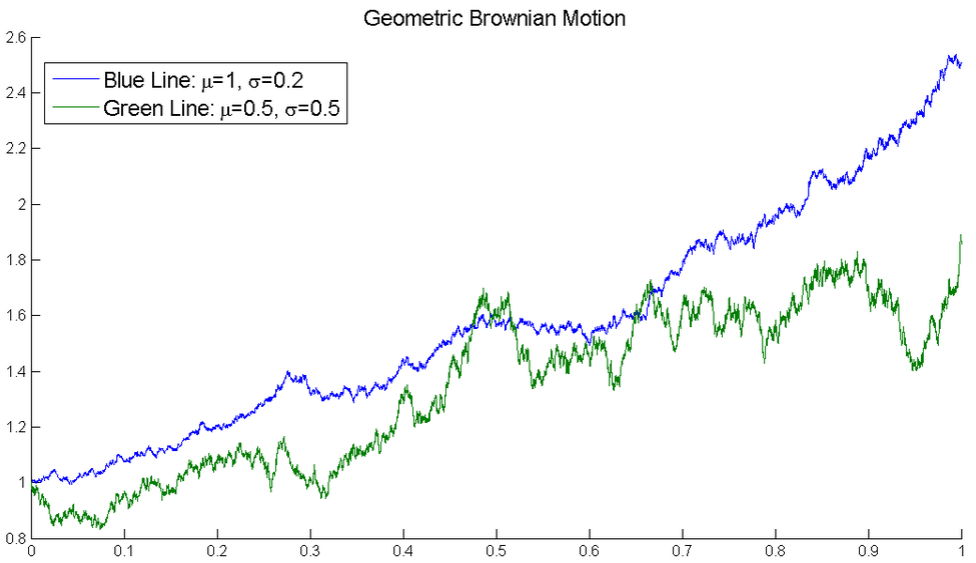
\includegraphics[width=8cm]{images_1/17.png}\\
			\caption{}\label{fig15}
		\end{figure}
		
	}
	
	\frame{\frametitle{布朗运动的应用}
		\parindent=19pt	
		\renewcommand{\raggedright}{\leftskip=0pt \rightskip=0pt plus 0cm}
		\raggedright
		使用几何布朗运动来描述股票价格的理由:
		\begin{itemize}
			\item 几何布朗运动的期望与随机过程的价格(股票价格)是独立的, 这与我们对现实市场的期望是相符的。
			\item 几何布朗运动过程与我们在股票市场观察到的价格轨迹呈现了同样的“roughness” 。
			\item 几何布朗运动过程计算相对简单。
		\end{itemize}
		
		使用几何布朗运动来描述股票价格的缺陷:
		\begin{itemize}
			\item 在真实股票价格中波动随时间变化, 但是在几何布朗运动中, 波动是不随时间变化的。
			\item 在真实股票价格中, 收益通常不服从正态分布。
		\end{itemize}
		
	}
	
	\frame{\frametitle{布朗运动的其他应用}
		\parindent=19pt	
		\renewcommand{\raggedright}{\leftskip=0pt \rightskip=0pt plus 0cm}
		\raggedright
		\begin{itemize}
			\item 研究仪器的灵敏度:在近代无线电技术 (如卫星通讯 ) 中,由于放大倍数很高,电涨落现象表现得特别显著,引起热噪声,这个问题也需要用布朗运动理论来研究。
			\item 研究各类扩散现象:扩散现象的本质是布朗运动产生的位移,因此布朗运动理论可用于各类扩散现象。例如半导体 中载流子 (电子或空穴 ) 的扩散,原子核反应堆中中子的扩散等,均可用布朗运动理论来研究。
			\item 分形布朗运动模型在地形分析、模式识别、数字图像处理、信息讯号的处理中的应用。
			\item 1990年以来,量子布朗运动理论进一步发展,转向对纳米结构中粒子运动和生物细胞中分子机器的研究。
		\end{itemize}
	}
	
%	\begin{frame}\fontsize{30pt}{30pt}\selectfont
	%\begin{center}
	%		谢谢!
	%	\end{center}
%	\begin{figure}
%		\centering
		% Requires \usepackage{graphicx}
%		
\includegraphics[width=6cm]{images/12.jpg}\\
%		\caption{}\label{fig12}
%	\end{figure}
	
%\end{frame}




%Random Walk 2
\section{随机游走}
	
	\frame{
		\centerline{\textbf{\Huge{随机游走}}}
	}
	
	\frame{\frametitle{定义}
		
		随机游走(random walk)也称随机漫步,随机行走等是指基于过去的表现,无法预测将来的发展步骤和方向。核心概念是指任何无规则行走者所带的守恒量都各自对应着一个扩散运输定律 ,接近于布朗运动,是布朗运动理想的数学状态,现阶段主要应用于互联网链接分析及金融股票市场中。
	}
	
	\frame{\frametitle{思想}
		
		全局最优化,操作简单,不易陷入局部极小值
	}
	
	\frame{\frametitle{思想}
		\begin{itemize}
			\item<1-> 全局最优化:目前还没有一个通用的办法可以对任意复杂函数求解全局最优值。
			\item<2-> 操作简单:易于依托代码实现该算法。
			\item<3-> 不易陷入局部极小值:源于算法中的不断迭代过程。
		\end{itemize}
	}
	
	\frame{\frametitle{算法流程}
		\begin{itemize}
			\item<1-> 设f(x)是一个含有n个变量的多元函数,x=(x1,x2,...,xn)为n维向量。
			\item<2-> 给定初始迭代点x,初次行走步长$\lambda$,控制精度$\epsilon$。
			\item<3-> 给定迭代控制次数N,k为当前迭代次数,置k=1。
			\item<4-> 当k<N时,随机生成一个(−1,1)之间的n维向量u=(u1,u2,⋯,un),(−1<ui<1,i=1,2,⋯,n)。
			\item<5-> 将n维向量标准化得到
			\begin{equation} 
			\label{eqn15} 
			u' =\frac{u}{\sqrt{\sum_{i=1}^nu_{i}^2}}
			\end{equation}
			\item<6-> 令
			\begin{equation} 
			\label{eqn16} 
			x_1 =x + \lambda u'
			\end{equation}从而完成第一步游走。
		\end{itemize}
	}
	
	\frame{\frametitle{算法流程}
		\begin{itemize}
			\item<1-> 计算函数值,如果 f(x1)<f(x),即找到了一个比初始值好的点,那么k重新置为1,将x1变为x,回到第2步;否则k=k+1,回到第3步。
			\item<2-> 如果连续N次都找不到更优的值,则认为,最优解就在以当前最优解为中心,当前步长为半径的N维球内。
			\item<3-> 此时,如果$\lambda<\epsilon$,则结束算法;否则,令$\lambda$减半,回到第1步,开始新一轮游走。
		\end{itemize}
	}
	
%3
\section{Heavy-tailed Distribution And Light-tailed Distribution}	

	\frame{
	\begin{center}
{\tnewroman \textbf{\Huge{Heavy-tailed Distribution And Light-tailed Distribution}}}
	\end{center}	
}
\begin{frame}

\frametitle{承前启后}
\qquad 如果捕食者像无头苍蝇一样漫无目的的做布朗运动,真的能很有效的地寻到到猎物吗?在数学上可以证明,布朗运动和分子自由扩散一样,单位速度的分子在时间$t$内平均只有$\sqrt{t}$的位移量。若捕食者采用这种策略,需要很久才能够成功。

\qquad 那么有没有比布朗运动更高效的搜索方法呢?一组巴西物理学家于$1999$年提出了一个设想,认为“莱维飞行”比布朗运动有更高的搜索效率,因此自然会偏向与采用“莱维飞行”捕食的生物。为了理解什么是“莱维飞行”,我们首先需要对概率分布的轻尾性和重尾性有一个认识。
%\tableofcontents

\end{frame}
	
\begin{frame}
\frametitle{指数分布}
指数分布是描述泊松过程中的事件之间的时间的概率分布,即事件以恒定平均速率连续且独立地发生地过程。它是几何分布的
连续模拟,它具有无记忆的关键性质。例如,如果T是某一元件的寿命,已知元件使用了$t$小时,它总共使用至少$s+t$小时的条件概率与一开始使用时算起它使用至少s小时的概率相等。

其概率密度函数:

\begin{displaymath}
F\left ( x;\lambda  \right )= \left\{\begin{matrix}
1-e^{-\lambda x}, &x\geq 0  \\
0, &x< 0
\end{matrix}\right.
\end{displaymath}

\end{frame}

\begin{frame}
\frametitle{轻尾分布}
\qquad 比指数分布尾部更薄的概率分布是轻尾分布。 它们下降到$0$的速度比指数分布的速度快得多,因此在尾部质量更小。 Gumbel 分布是轻尾分布的一个例子。轻尾分布并不能很好地反映“真实世界”的数据。



\centering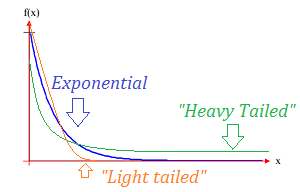
\includegraphics[scale=0.5]{image/light-tailed.png}


\end{frame}

\begin{frame}

\frametitle{概率分布的轻尾性}
\qquad 前面说过,布朗运动的步长服从正态分布。正态分布是一种典型的{\color{red}{轻尾分布}}, 也就是说,不太可能取得极端值的分布。

\begin{figure}
	\centering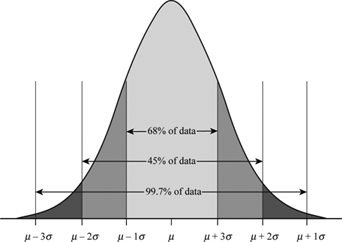
\includegraphics[scale=0.35]{image/normal_distribution.png}
\end{figure}

表达式$y= \frac{1}{\sqrt{2\pi}\sigma}e^{\frac{-\left ( x-\mu  \right )^{2}}{2\sigma ^{2}}}$。其中$\mu$是均值,$\sigma$是标准差。当$x$增大
时,函数下滑趋势非常快,因此数学家又将正态分布函数纳入速降函数空间范畴。速降函数是专门为傅里叶分析而量身定做的。
%\begin{definition}
%    definition 1...
%\end{definition}

\end{frame}

\begin{frame}

\frametitle{概率分布的重尾性}
\qquad 而在现实生活中,大多数的事情不能用轻尾分布来描述,例如保险领域的保险金-事故可以看作是稀有事件,但一旦发生并通过审核,保险公司就必须大量金额,这样一来保险金的分布就很可能取到很大的值。为了描述这样容易取得极值的随机变量,我们需要引入重尾分布。

\centering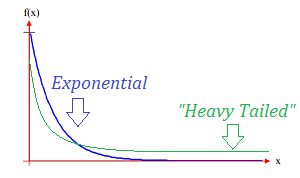
\includegraphics[scale=0.5]{image/heavy_tailed.png}

典型特点: 大头短$+$小尾长。“莱维飞行”的平均位移是$t^{\gamma}$,$\gamma>\frac{1}{2}$.
\end{frame}
\begin{frame}
\frametitle{重尾分布}
当$x\rightarrow \infty$时,重尾分布下降到$0$的速度慢于指数分布。因而尾部质量较大。其数学定义为:

\begin{displaymath}
\lim_{x\rightarrow \infty }e^{\lambda x}F\left ( x \right )=\infty
\end{displaymath}

其中,$\lambda>0$, $F(x)$是尾分布函数。

重尾分布更适用于对那些离峰值较远的稀有事件也会有相当的概率发生的情况。重尾分布作为一个大的类别,还包含三个重要的子类别,分别是肥尾分布(Fat-tailed distribution),长尾分布(Long-tailed distribution)和次指数分布(Subexponential distribution)
\end{frame}

\begin{frame}

\frametitle{概率分布的重尾性}
\qquad 那么,如何验证“莱维飞行”的有效性呢?一个方案就是前面提到的大肠杆菌的{\color{red}{趋化行为}}。尽管最初的“莱维飞行”假说是针对动物
而言的,但从大肠杆菌的游击战策略可以看出,该假说对微生物同样适用!这样一来,对微生物的研究也能反过来帮助人们更深入地理解动物行为,这便是微观的细胞生物学在宏观的生态学中的应用。

\end{frame}

\begin{frame}
\frametitle{莱维过程}
\qquad 莱维过程$\left \{ X\left ( t \right ),t\geq 0 \right \}$是一种随机过程,它满足的条件比布朗运动宽松:
\begin{itemize}
\item $X{0}$ 几乎处处为0;
\item 独立增量性;
\item 稳定增量性;
\item 样本轨道右连续.
\end{itemize}


\qquad 连续的布朗运动和离散的泊松过程都是莱维过程的特例。因此可以大胆猜测,莱维过程就是带“跳跃”的布朗运动。正是这些不连续
性的“跳跃”给予莱维过程“重尾”的特性。
\end{frame}
	
	
	
	
%Levy 4
\section{莱维过程}
	\frame{
	\centerline{\textbf{\Huge{莱维过程}}}
}

%\section{定义}
\begin{frame}
\frametitle{定义}
一个随机过程 ${X=\{X_{t}:t\geq 0\}}$如果符合以下条件: 
\begin{enumerate}[(1)]
\item $X_{0}=0$.
\item 独立增量:对于任何$0\leq t_{1} < t_{2} < \dots < t_{n} < \infty ,X_{t_2}-X_{t_1},X_{t_3}-X_{t_2},\dots,X_{t_n}-X_{t_{n-1}}$相互独立.
\item 稳定增量:对任何s<t, $X_{t}-X_{s}$ 与 $X_{t-s}$有相同分布 .  
\item X几乎确定是右连左极.
\end{enumerate}
我们把X称作levy过程.
\end{frame}

%\section{无限可分分布(infinitely divisible distribution)}
\begin{frame}
\frametitle{无限可分分布(infinitely divisible distribution)}
\begin{itemize}
\item 定义:对于一个随机变量U,如果存在一系列的独立同分布的随机变量$U_{1,n},\dots,U_{n,n}$,使得U$\overset{\text{d}}{=}U_{1,n}+\dots+U_{n,n}$,那么随机变量U拥有无限可分分布,$\overset{\text{d}}{=}$意味着同分布.
\item 如果U是一个随机变量,那么它的特征函数h:R $\to$ C为:h($\theta$)=E[$e^{i\theta U}$],$\theta \in R$.
\item U是一个无限可分随机变量,h是特征函数,那么:
\begin{enumerate}[(1)]
\item h是连续并且非0的,h(0)=1.
\item 存在一个独特的连续函数,对于所有$\theta \in R$满足$e^{f(\theta)}=h(\theta)$,f是U的特征指数
\end{enumerate}
\end{itemize}
\end{frame}

\begin{frame}
定理:如果X是一个levy过程,对于任何$t \geq 0$,随机变量 $X_{t_1} $ 拥有无限可分分布.
证明:如果X是kevy过程,并且$t \geq 0$.那么对于n=1,2,\dots,\[ X_{t}=X_{t/n}+(X_{2t/n}-X_{t/n})+\dots+(X_{t}-X_{(n-1)t/n})\]右边的每项都是独立同分布,并且有独立稳定增量属性,因此,${X_{t}}$拥有无限可分分布.
接下来,我们看下一维levy过程的特征函数,对于levy过程X,$X_{t}$的特征指数为$\psi_{t}$,\[e^{\psi_{t}(\theta)}=E[e^{i \theta X_{t}}] ,\theta \in R \]通过上面的公式,我们可以得到\[ m\psi_{1}(\theta)=\psi_{m}(\theta)=n\psi_{m/n}(\theta)\] 也就是说对于$t \geq 0$,\[\psi_{t}(\theta)=t\psi_{1}(\theta)\]因此,我们可以得到\[E[e^{i\theta X_{t}}]=e^{t\psi(\theta)}, \theta \in R\]其中,$\psi$:=$\psi_{1}$是$X_{1}$的特征指数.

\end{frame}
%\section{莱维-辛钦定理}
\begin{frame}
\frametitle{莱维-辛钦定理}
莱维-辛钦定理:X为levy过程,特征指数为$\psi$.存在唯一的$a \in R,\sigma \geq 0$以及测度$\prod$,满足$\int_R 1 \bigwedge x \prod \,dx$  \[\psi(\theta)=ia\theta-\frac{1}{2}\sigma_{2}\theta_{2}+(\int_R e^{i\theta x}-1-i\theta xI_{[-1,1]}(x))\prod(dx) \, \]对于上述三个参数($a,\sigma,\prod$),a包含了任何确定的漂移项,$\sigma$是高斯系数,描述了布朗运动的波动性,而$\prod$描述了X跳跃的大小和强度
\end{frame}

%\section{levy过程的特例}
\begin{frame}
\frametitle{possion 过程}
possion过程的概率密度函数为$\mu_{\lambda({k})}=e^{-\lambda}\lambda^{k}/k!$,因此possion分布的特征函数为\[\sum_{k=1}^{n}e^{i\theta k}\mu_{\lambda}({k})=e^{\lambda(e^{i\lambda}-1)}=[e^{\frac{\lambda}{n}(e^{i\theta}-1)]^{n}} \]因此对于一个possion过程{$N_{t}:t \geq 0$}如果参数为$\lambda t$,则是levy过程,特征函数为$E(e^{i\theta N_{t}})=e^{\lambda t(e^{i\theta}-1)}$,特征指数为$\psi(\theta)=\lambda(e^{i\theta}-1)$
\end{frame}

\begin{frame}
复合possion过程\newline\newline
N为possion过程,对于$\theta \in R $,特征函数为\[E(e^{i\theta\sum_{i=1}^{N}\xi_{i}})=\sum_{n\geq0}E(e^{i\theta\sum_{i=1}^{N}\xi_{i}})e^{-\lambda}\frac{\lambda^{n}}{n!}\]
\newline
\[=\sum_{n\geq0}(\int_R e^{i\theta x}F(dx)\,)^{n}e^{-\lambda}=e^{\lambda\int_R e^{i\theta x}F(dx)\,} \]其中三个参数分别为$a=\lambda\int_{0<|x|<1}xF(dx) \,$,$\sigma=0$,$\prod(dx)=\lambda F(dx)$.

\end{frame}

\begin{frame}
布朗运动\newline\newline
布朗运动的概率密度函数为:\[\mu_{s,\gamma}(dx):=\frac{1}{\sqrt{2\pi s^{2}}}e^{-(x-\gamma)^{2}/2s^{2}}dx ,x \in R\]我们可以得到他的特征函数和特征指数:\[E[e^{i\theta U}]=e^{\frac{1}{2}s^{2}\theta^{2}+i\theta\gamma}\]三个参数为$a=-\gamma,\sigma=s,\prod=0$

\end{frame}

%\section{莱维-伊藤分解}
\begin{frame}
\frametitle{莱维-伊藤分解}


根据莱维-辛钦定理,我们可以得到如下公式\[\Psi(\theta)=\{ia\theta+\frac{1}{2}\sigma^{2}\theta^{2}\}+\{\prod(R\backslash(-1,1))\int_{|x|\geq1}(1-e^{i\theta x})\frac{\prod{dx}}{\prod(R\backslash(-1,1)} \,\}\]\newline\[+\{\int_{0<|x|<1}(1-e^{i\theta x}+i\theta x)\prod(dx) \,\} \]
第一项是线性布朗运动,第二项是复合泊松过程,第三项是平方可积鞅.因此levy过程可由这三个过程组合而成.

\end{frame}



\section{分解定理}\fontsize{10pt}{10pt}\selectfont

\frame{
	\centerline{\textbf{\Huge{分解定理}}}
}
\frame{\frametitle{背景}
	\parindent=19pt	
	\renewcommand{\raggedright}{\leftskip=0pt \rightskip=0pt plus 0cm}
	\raggedright
	细菌觅食算法(BFA)由K. M. Passino于2002年基于Ecoli大肠杆菌在人体肠道内吞噬食物的行为,提出一种新型仿真算法,该算法属于随机搜索算法。该算法因具有群体智能算法并行搜索、易于跳出局部极小值、对初值和参数选择要求低、鲁棒性好、全局搜索等优点,成为生物启发式计算研究领域的又一热点。
	\begin{figure}[H]
		\centering
		% Requires \usepackage{graphicx}
		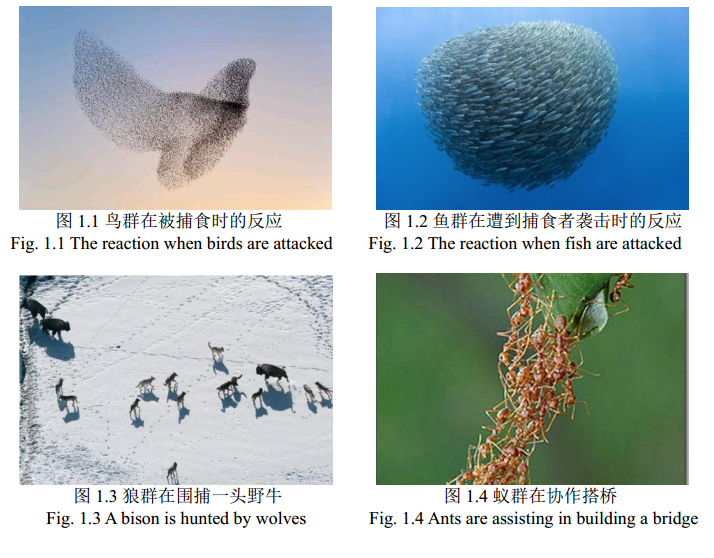
\includegraphics[width=6cm]{figure/1.png}\\
		\caption{群体智能}\label{fig1}
	\end{figure}
	
}

\frame{\frametitle{大肠杆菌特点}
	\parindent=19pt	
	\renewcommand{\raggedright}{\leftskip=0pt \rightskip=0pt plus 0cm}
	\raggedright	
	基于大肠杆菌生物模型理论,算法主要融合了大肠杆菌的趋化行为、复制行为、迁徙行为和描述生物群体感应机制的聚集行为。大肠杆菌是一种常见的普通原核生物,由细胞膜、细胞壁、细胞质和细胞核等构成,其两端钝圆呈杆状。表面布满纤毛和鞭毛。纤毛是一种呈凸起状且可运动的细胞器,通过纤毛向彼此传递消息。
	\begin{figure}
		\centering
		% Requires \usepackage{graphicx}
		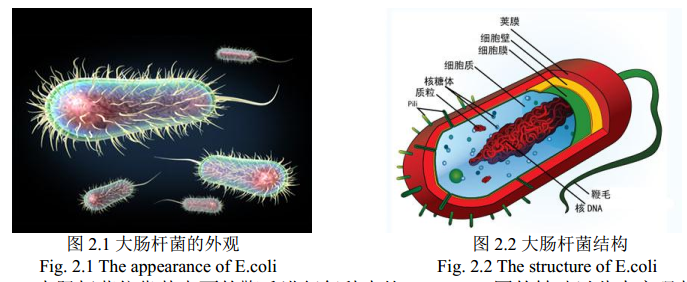
\includegraphics[width=8cm]{figure/2.png}\\
		\caption{大肠杆菌模型}\label{fig2}
	\end{figure}
	
}
\frame{\frametitle{大肠杆菌特点}
	\parindent=19pt	
	\renewcommand{\raggedright}{\leftskip=0pt \rightskip=0pt plus 0cm}
	\raggedright	
	大肠杆菌依靠其表面的鞭毛进行每秒大约100~200圈的转动以此来实现其自身的运动,当鞭毛逆时针摆动时,会给细菌一个向前的推力保证其向前游走;而当鞭毛进行顺时针摆动时,会给其一个拉力其细菌翻转。大肠杆菌正是通过游动和翻转这两个基本动作组合来实现其在空间区域中的移动。
	\begin{figure}
		\centering
		% Requires \usepackage{graphicx}
		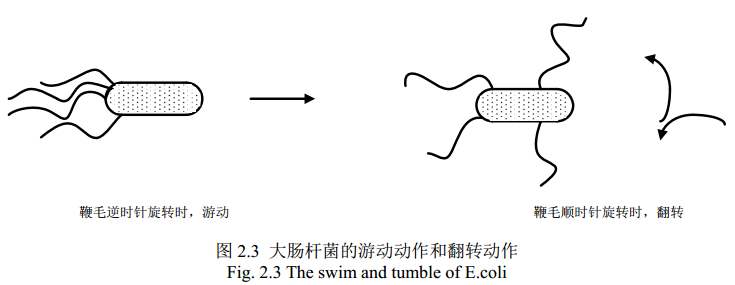
\includegraphics[width=8cm]{figure/3.png}\\
		\caption{大肠杆菌运动模型}\label{fig3}
	\end{figure}
	
}

\frame{\frametitle{大肠杆菌特点}
	\parindent=19pt	
	\renewcommand{\raggedright}{\leftskip=0pt \rightskip=0pt plus 0cm}
	\raggedright	
	大肠杆菌虽是一种简单的生物,但对所经历的周围环境具有记忆其状态的能力,这种能力帮助大肠杆菌在搜索食物的过程中避开有毒物质向着存在食物的方向运动。同时,大肠杆菌也会对所经历过的所有状态都行评价据此反馈信息给后面的状态改变。包括周围环境的物理、化学因素变动所引起的温度过高、营养匮乏、环境PH值过偏等;也包括细菌本身的生理代谢过程也会使得所处环境发生变化。区域细菌浓度也是信号之一。
	\begin{figure}
		\centering
		% Requires \usepackage{graphicx}
		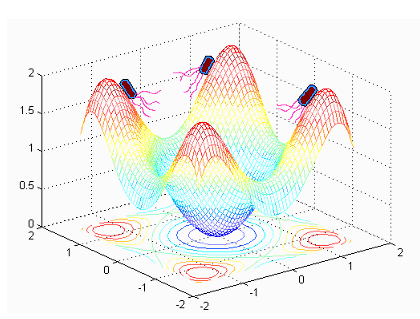
\includegraphics[width=6cm]{figure/8.png}\\
		\caption{应用示意图}\label{fig8}
	\end{figure}
	
}

\frame{\frametitle{大肠杆菌特点}
	\parindent=19pt	
	\renewcommand{\raggedright}{\leftskip=0pt \rightskip=0pt plus 0cm}
	\raggedright	
	通常食物是分布在多个区域之中的。首先,大肠杆菌利用自己的鞭毛进行游动来搜索食物的潜在区域。然后大肠杆菌决定是否进入选择的目标区域,若不进入,则继续搜索。当进入一个目标区域后,如果食物丰富,则停留至食物耗尽,之后沿着上次前进的方向继续搜索食物;如若该区域食物匮乏,那么细菌将会改变前进方向,朝着可能食物丰富区域搜索。
	\begin{figure}
		\centering
		% Requires \usepackage{graphicx}
		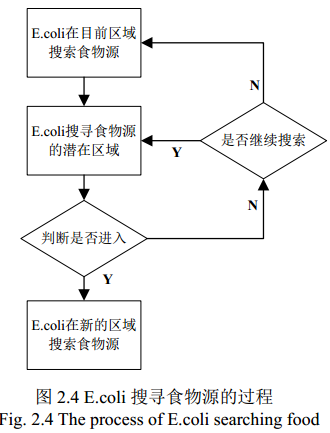
\includegraphics[width=4cm]{figure/4.png}\\
		\caption{大肠杆菌搜索食物流程图}\label{fig4}
	\end{figure}
	
}


\frame{\frametitle{算法基本原理}
	\parindent=19pt	
	\renewcommand{\raggedright}{\leftskip=0pt \rightskip=0pt plus 0cm}
	\raggedright
	大肠杆菌自身的引导控制系统来趋利避害。算法中待求解优化问题的解空间对应为细菌觅食的整个搜索空间,各个优化问题的解则对应为细菌在空间中的位置,那么最优解总是被由更好食物源位置所对应的更好的优化问题解所不断靠近。
	\begin{figure}
		\centering
		% Requires \usepackage{graphicx}
		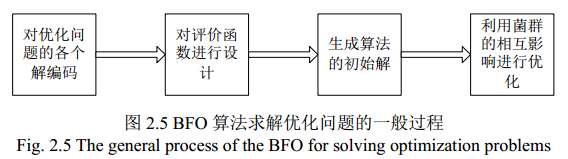
\includegraphics[width=8cm]{figure/5.png}\\
		\caption{求解过程}\label{fig5}
	\end{figure}
	
}

\frame{\frametitle{算法基本原理}
	\parindent=19pt	
	\renewcommand{\raggedright}{\leftskip=0pt \rightskip=0pt plus 0cm}
	\raggedright
	细菌觅食算法是随机搜索的智能优化算法,其数学模型主要有三个基本步骤:趋向、复制、迁移。几何解释为三个循环层操作,最里层是趋向,中间层是复制,最外层是迁移。细菌觅食主要就是依据这三层循环操作来寻找食物。
}
\frame{\frametitle{算法基本原理}
	\parindent=19pt	
	\renewcommand{\raggedright}{\leftskip=0pt \rightskip=0pt plus 0cm}
	\raggedright
	其觅食特点依靠鞭毛的旋转方向,逆时针,快速前进;顺时针,则停留原地。相应的数学模型解释就是当计算出两个点位置的函数的适应度值,通过比较结果决定大肠杆菌是继续前进还是寻找随机方向移动,当尝试次数达到最大限制数时选择下一个大肠杆菌进行趋向性操作。其数学表达式为
	\begin{equation}
	\theta^{'}(j+1,k,l)=\theta^{'}(j,k,l)+C(i)\frac{\Delta(i)}{\sqrt{\Delta(i)^T\Delta(i)}}
	\end{equation}
	其中$\theta^{'}(j,k,l)$表示大肠杆菌$i$在第$j$次趋向第$k$次复制第$l$次迁移操作之后所在的位置,$C(i)$为趋向步长,$\frac{\Delta(i)}{\sqrt{\Delta(i)^T\Delta(i)}}$为移动的一个随机前进方向。
}
\frame{\frametitle{算法基本原理}
	\parindent=19pt	
	\renewcommand{\raggedright}{\leftskip=0pt \rightskip=0pt plus 0cm}
	\raggedright
	自然界生物进化的准则是优胜劣汰,因此性能差的细菌会被淘汰。在BFA模型中,$J(i,j,k,l)$表示细菌$i$在第$j$次趋向第$k$次复制第$l$次迁移操作之后的适应值。$J_{health}^i$是细菌$i$的能量函数,其大小决定细菌觅食能力的强弱。将觅食后的细菌的能量函数进行大小排序,淘汰掉$\frac{S}{2}$个能量值较小的细菌,将剩下的进行赋值操作,新生成的复制细菌与原细菌具有相同的觅食能力。
	
}
\frame{\frametitle{算法基本原理}
	\parindent=19pt	
	\renewcommand{\raggedright}{\leftskip=0pt \rightskip=0pt plus 0cm}
	\raggedright
	在生物体中存在的细菌,其环境对其觅食具有很大的影响,比如局部区域温度升高或者食物被消耗掉,这些必然导致细菌被迫迁移到新的区域去寻找食物。这种迁移未必会导致细菌寻找不到新的食物,反而会对种群的良好生长起到促进作用,在经过复制操作之后细菌若按照一定的概率进行迁移,新的种群具有随机特性,与原种群相比可能有不同的觅食能力,这种随机性能使群体跳出局部极值而更好的靠近全局最优解区域。
	
}
\frame{\frametitle{算法基本原理}
	\parindent=19pt	
	\renewcommand{\raggedright}{\leftskip=0pt \rightskip=0pt plus 0cm}
	\raggedright
	在细菌觅食过程中,并不是独立行为,即在模型中体现为引力和斥力,当引力作用是,细菌会快速的聚集在一起,围绕最优食物觅食,形成细菌群。当斥力起作用时,表示细菌能具有更好的独立寻找食物的能力。其数据模型为
	\begin{equation}
	\begin{split}
	J_{cc}(\theta,P(j,k,l))&=\sum_{i=1}^SJ_{cc}(\theta,\theta^i(j,k,l))\\
	&=\sum_{i=1}^S[-d_{att}\exp(-\omega_{att}\sum_{m=1}^P(\theta-\theta_m^i)^2)]\\
	&+\sum_{i=1}^S[h_{rep}\exp(-\omega_{rep}\sum_{m=1}^P(\theta-\theta_m^i)^2)]
	\end{split}
	\end{equation}
	其中$d_{att}$是引力深度,$\omega_{att}$是引力宽度,$h_{rep}$是斥力高度,$\omega_{rep}$是斥力宽度,$\theta_m^i$是细菌$i$的第$m$个分量。通常取$d_{att}=h_{rep}$,趋向性操作的适应度值的计算公式可表示为:
	\begin{equation}
	J(i,j+1,k,l)=J(i,j,k,l)+J_{cc}(\theta^i(j+1,k,l),P(j+1,k,l))
	\end{equation}
}
\frame{\frametitle{算法主要步骤}
	\parindent=19pt	
	\renewcommand{\raggedright}{\leftskip=0pt \rightskip=0pt plus 0cm}
	\raggedright
	
	Step1:初始化参数,种群大小$S$,空间维数$P$,趋向性行为的次数$N_c$,趋向性操作前进最大步数$N_s$,复制性操作的次数$N_{re}$,迁移操作的次数$N_{ed}$,迁移概率$P_{ed}$,细菌$i$的信息用$D$维向量表示为$\theta^i=[\theta_1^i,theta_2^i,...,\theta_D^i],i=1,2,...,S,$趋向性步长$C(i)$.
	
	Step2:迁移循环操作;
	
	Step3:复制循环操作;
	
	Step4:趋向性循环操作;
	
	(1)细菌$i$进行趋向性一步;
	
	(2)计算$J(i,j,kl)$,储存最优值$J_{best}$;
	
	(3)随机生成向量$\Delta(i)$,细菌按照步长$C(i)$进行移动;
	
	(4)计算此时的适应度值$J(i,j+1,k,l)$;
	
	(5)旋转判定条件:若$m<N_s,m=m+1$,若$J(i,j+1,k,l)<J_{best}$,则$J_{best}=J(imj+1,k,l)$,此时$\theta^i(j+1,k,l)=\theta^i(j,k,l+C(i)\frac{\Delta(i)}{\sqrt{\Delta(i)^T\Delta(i)}}$.根据细菌的信息量$\theta^i(j+1,k,l)$计算新的$J(j+1,k,l)$否则$m=N_s$.
	
	(6)重新处理下一个细菌。
	
	
}


\frame{\frametitle{算法主要步骤}
	\parindent=19pt	
	\renewcommand{\raggedright}{\leftskip=0pt \rightskip=0pt plus 0cm}
	\raggedright
	
	Step5:若$j<N_c$返回上一步进行细菌趋向性操作。
	
	Step6:复制,淘汰$\frac{S}{2}$个能量值小的细菌,对剩下的$\frac{S}{2}$个细菌进行复制。
	
	Step7:若$k<N_{re}$,返回Step3.
	
	Step8:迁移,达到一定条件后细菌以概率$P_{ed}$重新觅食。若$l<N_d$,则返回Step2,否则寻优结束。
	
	Step9:循环结束条件判断,条件满足则结束,输出结果。
}
\frame{\frametitle{参数选取}
	\parindent=19pt	
	\renewcommand{\raggedright}{\leftskip=0pt \rightskip=0pt plus 0cm}
	\raggedright
	
	模型中种群的规模$S$太大导致计算量增大,太小会降低种群的多样性;趋向性步长$C$太大时,优化值易陷入局部极值;当太小时,算法的计算复杂度会大幅度增加,不利于算法收敛;引力参数$d_{att}$和$\omega_{att}$大小决定算法的群聚性,如果值较大会导致不按照自己的信息搜索寻找食物而过度的向中心靠拢,反之太小会完全按照自身信息搜索食物导致群聚性能很弱,斥力参数$h_{rep},\omega_{rep}$与引力参数相反;趋向性操作因子$N_c$决定算法的寻优能力和收敛速度;趋向性参数$N_s$最大步长对算法的收敛速度有很大的影响;赋值操作因子$N_{re}$决定算法的计算复杂度和收敛速度,并且复制操作所采取的原则计算出的适应度值只与当前位置有关,导致最优解被淘汰掉容易陷入局部最优;迁移操作因子执行次数$N_{ed}$太小会使算法陷入局部最优,反之计算量和复杂度增加,迁移概率$P_{ed}$太大会使算法进入循环搜索,以至远离最优解。
	
}
\frame{\frametitle{案例}
	\parindent=19pt	
	\renewcommand{\raggedright}{\leftskip=0pt \rightskip=0pt plus 0cm}
	\raggedright	
	对优化问题$\min\sum_{i=1}^nx_i^2+x_i$做测试。
	\begin{figure}
		\centering
		% Requires \usepackage{graphicx}
		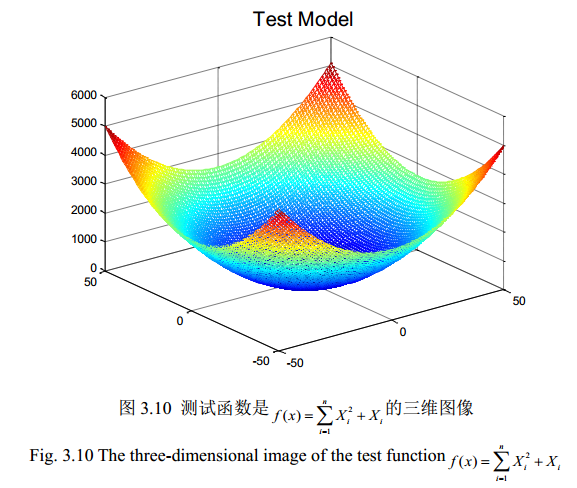
\includegraphics[width=8cm]{figure/6.png}\\
		\caption{测试案例}\label{fig6}
	\end{figure}
	
}

\frame{\frametitle{仿真结果}
	\parindent=19pt	
	\renewcommand{\raggedright}{\leftskip=0pt \rightskip=0pt plus 0cm}
	\raggedright
	对算法进行10000次仿真。对如下四个标志数据:最小值、最大值、平均值、标准差等做评价。
	\begin{figure}
		\centering
		% Requires \usepackage{graphicx}
		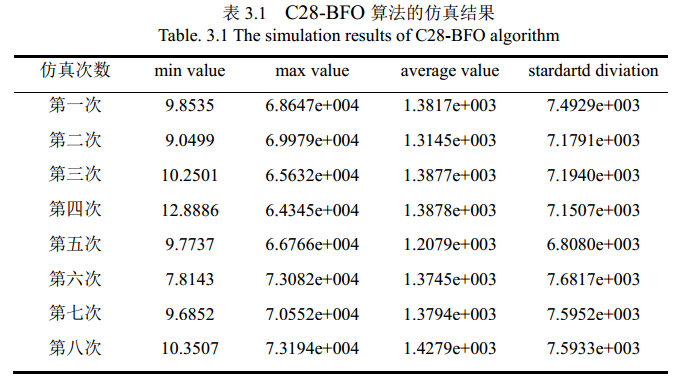
\includegraphics[width=8cm]{figure/7.png}\\
		\caption{测试结果}\label{fig7}
	\end{figure}
	
}

\frame{\frametitle{算法应用}
	\parindent=19pt	
	\renewcommand{\raggedright}{\leftskip=0pt \rightskip=0pt plus 0cm}
	\raggedright
	在控制领域主要是控制器设计,可以用细菌觅食算法求解PID控制器参数优化问题。同样,BFA在图像处理领域中得到很好的应用,主要应用于图像分割、边缘检测、图像压缩等。亦可将细菌觅食算法应用到神经网络学习机制中,应用到负荷预测。也可通过BFA来优化模糊系统的参数,优化后的滤波器优于传统的卡尔曼滤波器。在盲信号分离也可应用BFA,在模式识别领域得到广泛探索。此外,细菌觅食算法在调度问题、股票经济预测、组合优化等问题中也有广泛应用。
}
\frame{\frametitle{觅食策略}
	\parindent=19pt	
	\renewcommand{\raggedright}{\leftskip=0pt \rightskip=0pt plus 0cm}
	\raggedright	
	多说站在食物链顶端的动物们,例如狮子、老虎等主要靠视觉来搜寻猎物,和靠气味觅食(大白鲨)不同,视觉不存在所谓的梯度差,看不见就是看不见,没有动物具有透视眼。所以觅食策略对于狮子老虎这样的陆地动物是很重要的。在不知道猎物位置的情况下,\textcolor{red}{布朗运动}或许是最自然的方法了。布朗运动是一个随机过程,它的步长服从\textcolor{red}{正态分布}。
	
	离散版的布朗运动叫做\textcolor{red}{随机游走}(Random walk),它的步长和方向都是离散的。尽管布朗运动和随机游走是两个概念,也各自发展出了一套不同的理论,但两者的数学本质是一样的。
}

\frame{\frametitle{布朗运动轨迹}
	\parindent=19pt	
	\renewcommand{\raggedright}{\leftskip=0pt \rightskip=0pt plus 0cm}
	\raggedright	
	\begin{figure}
		\centering
		% Requires \usepackage{graphicx}
		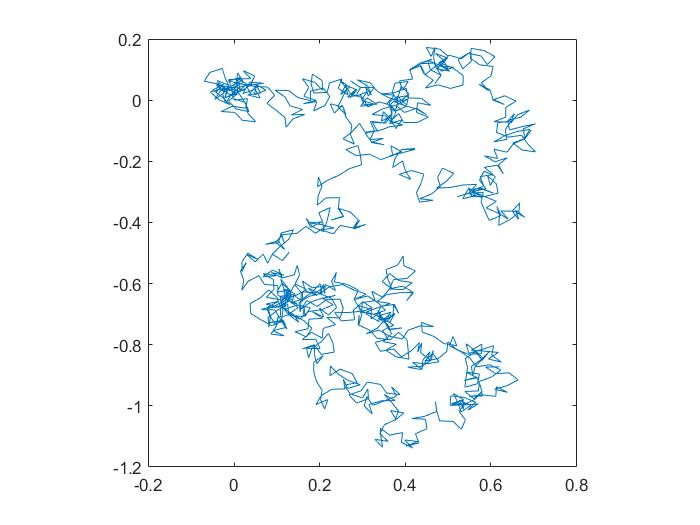
\includegraphics[width=8cm]{figure/14.jpg}\\
		\caption{布朗运动轨迹图}\label{fig14}
	\end{figure}
	现在提供一个布朗运动的轨迹图。
}

\frame{\frametitle{布朗运动}
	\parindent=19pt	
	\renewcommand{\raggedright}{\leftskip=0pt \rightskip=0pt plus 0cm}
	\raggedright	
	随机过程是一系列随机变量的集合。比如说,每丢一次硬币,便产生一个随机变量,那么一次次的丢下去,便产生一系列的随机变量$X_1,...,X_i,...$.随机变量序列集合起来,便是随机过程。
	
	布朗运动是悬浮在液体或气体中的微粒所作的永不停息的无规则运动。它是一种正态分布的独立增量连续随机过程。其基本性质为:布朗运动$W(t)$是期望为0,方差为$t$(时间)的正态随机变量。对于任意的$r\le s, w(t)-W(s)$独立于$W(r)$,且是期望为0方差为$t-s$的正态随机变量。
}
\frame{\frametitle{觅食策略}
	\parindent=19pt	
	\renewcommand{\raggedright}{\leftskip=0pt \rightskip=0pt plus 0cm}
	\raggedright	
	在物理学家眼里,布朗运动可以用\textcolor{red}{郎之万方程}(Langevin Equation。提出人保罗$\cdot$郎之万是法国物理学家,居里夫人丈夫皮埃尔$\cdot$ 居里的博士生,并且后来给皮埃尔$\cdot$居里戴了绿帽子)来描述:
	\begin{equation}
	m\frac{d^2x}{dt^2}=f(t)+F^{'}(t).
	\end{equation}
	其中$f(t)$分成两部分,一部分为阻力$-\alpha v$;一部分为随机作用力$F(t)$。 粘滞阻力仍来自介质分子对颗粒的碰撞,将颗粒看作半径为$a$的小球,在粘滞系数为$\eta$的流体中运动,则有$\alpha=6\pi\eta a$。
	\begin{equation}
	m\ddot{x}=-\mu \dot{x}(t)+\eta(t).
	\end{equation}
	其中$\eta(t)$是均值为0,方差为常数的随机过程。更确切地讲,是白噪声过程。
}



\frame{\frametitle{觅食策略}
	\parindent=19pt	
	\renewcommand{\raggedright}{\leftskip=0pt \rightskip=0pt plus 0cm}
	\raggedright	
	因此郎之万方程本质上就是考虑了\textcolor{red}{随机误差}的牛顿第二定律,这样的方程又叫做\textcolor{red}{随机微分方程}(Stochastic Differential Equation)。尽管郎之万是第一个提出随机过程的人,但作为物理学家,他更关心这些方程是否符合实际物理现象,而不关心数学上的严谨性。因此这种模型并没有立即受到数据家的重视。
	
	到了二十世纪中叶,日本数学家伊藤清和苏联数学家Stratonovich先后使用概率论的方法,把随机微分方程发展成严谨的数学概念。尽管如此,但两人对随机微分方程定义各有不同,这也显示了\textcolor{red}{随机性}和\textcolor{red}{确定性}的本质差异。此外,随机微分方程多用于对一些多样化现象进行建模,比如不停变动的股票价格、部分物理现象如热扰动等。
}

\frame{\frametitle{觅食策略}
	\parindent=19pt	
	\renewcommand{\raggedright}{\leftskip=0pt \rightskip=0pt plus 0cm}
	\raggedright	
	如果捕食者像无头苍蝇一样漫无目的的做布朗运动,真的能很有效的地寻到到猎物吗?在数学上可以证明,布朗运动和分子自由扩散一样,单位速度的分子在时间$t$ 内平均只有$\sqrt{t}$的位移量。捕食者若采用此种策略,可能需要踏遍千山万水才能成功了。
	
	那么有没有比布朗运动更高效的搜索方法呢?一组巴西物理学家于1999年提出了一个设想,认为“莱维飞行”比布朗运动有更高的搜索效率,因此自然会偏向与采用“莱维飞行”捕食的生物。为了理解什么是“莱维飞行”,我们首先需要对概率分布的重尾性有一个认识。
}

\frame{\frametitle{概率分布的轻尾性}
	\parindent=19pt	
	\renewcommand{\raggedright}{\leftskip=0pt \rightskip=0pt plus 0cm}
	\raggedright	
	前面说过,布朗运动的步长服从正态分布。正态分布是一种典型的\textcolor{red}{轻尾分布},也就是说,不太可能取得极端值的分布。
	\begin{figure}
		\centering
		% Requires \usepackage{graphicx}
		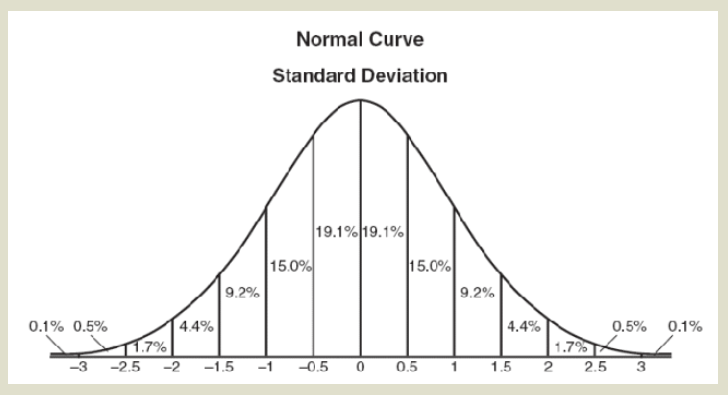
\includegraphics[width=8cm]{figure/9.png}\\
		\caption{正态分布图}\label{fig9}
	\end{figure}
	表达式:$y=\frac{1}{\sigma\sqrt{2\pi}}e^{\frac{-(x-\mu)^2}{2\sigma^2}}$。 其中$\mu$是均值,$\sigma$是标准差。当$x$增大时,函数下滑趋势可谓是猛如雪崩,因此数学家又将正态分布函数纳入速降函数空间范畴。速降函数是专门为傅里叶分析而量身定做的。
}
\frame{\frametitle{概率分布的重尾性}
	\parindent=19pt	
	\renewcommand{\raggedright}{\leftskip=0pt \rightskip=0pt plus 0cm}
	\raggedright	
	而在现实生活中,太多太多的事件不能用轻尾分布来描述,例如保险领域的保险金—— 事故可以看作是稀有事件,但一旦发生并通过审核,保险公司就必须大量金额,这样一来保险金的分布就很可能取到很大的值。为了描述这样容易取得极值的随机变量,我们需要引入\textcolor{red}{重尾分布}。
	\begin{figure}
		\centering
		% Requires \usepackage{graphicx}
		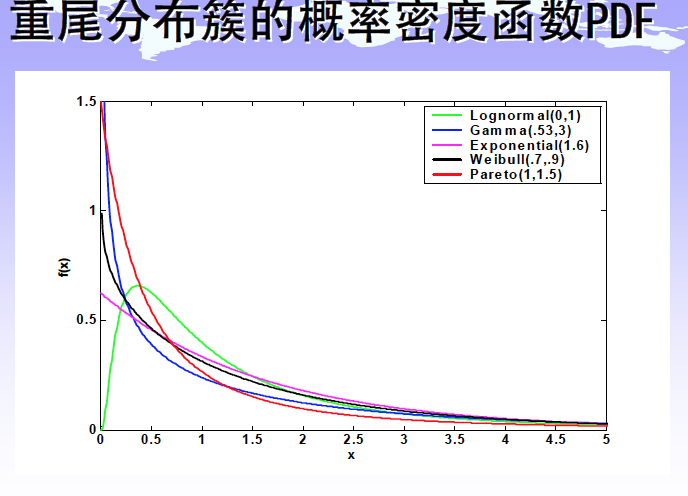
\includegraphics[width=8cm,height=4cm]{figure/10.png}\\
		\caption{重尾分布图}\label{fig10}
	\end{figure}
	典型特点:大头短+小尾长。“莱维飞行”的平均位移是$t^{\gamma},\gamma>\frac{1}{2}$。
}
\frame{\frametitle{概率分布的重尾性}
	\parindent=19pt	
	\renewcommand{\raggedright}{\leftskip=0pt \rightskip=0pt plus 0cm}
	\raggedright	
	那么,如何验证“莱维飞行”的有效性呢?一个方案就是前面提到的大肠杆菌的\textcolor{red}{趋化行为}。尽管最初的“莱维飞行”假说是针对动物而言的,但从大肠杆菌的游击战策略可以看出,该假说对微生物同样适用!这样一来,对微生物的研究也能反过来帮助人们更深入地理解动物行为,这便是微观的细胞生物学在宏观的生态学中的应用。
}
\frame{\frametitle{概率分布的重尾性}
	\parindent=19pt	
	\renewcommand{\raggedright}{\leftskip=0pt \rightskip=0pt plus 0cm}
	\raggedright	
	而在现实生活中,太多太多的事件不能用轻尾分布来描述,例如保险领域的保险金—— 事故可以看作是稀有事件,但一旦发生并通过审核,保险公司就必须大量金额,这样一来保险金的分布就很可能取到很大的值。为了描述这样容易取得极值的随机变量,我们需要引入\textcolor{red}{重尾分布}。
	\begin{figure}
		\centering
		% Requires \usepackage{graphicx}
		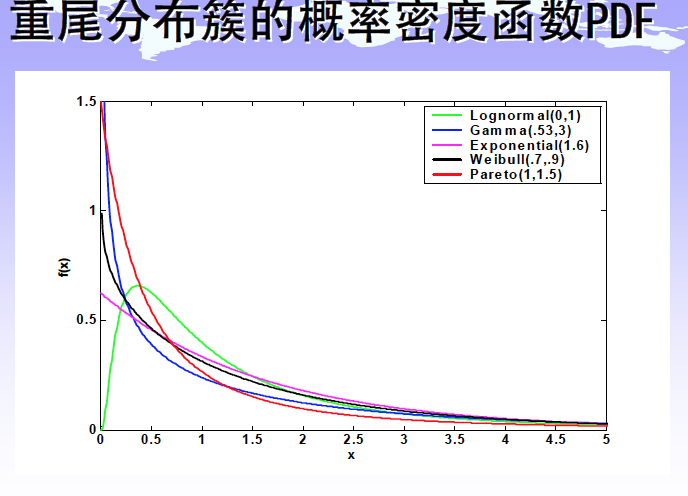
\includegraphics[width=8cm,height=4cm]{figure/10.png}\\
		\caption{重尾分布图}\label{fig10}
	\end{figure}
	典型特点:大头短+小尾长。“莱维飞行”的平均位移是$t^{\gamma},\gamma>\frac{1}{2}$。
}
\frame{\frametitle{莱维飞行}
	\parindent=19pt	
	\renewcommand{\raggedright}{\leftskip=0pt \rightskip=0pt plus 0cm}
	\raggedright	
	莱维飞行时服从莱维分布的随机搜索路径,是一种短距离的搜索与偶尔长距离的行走相间的行走方式,它能够解释很多自然现象,如布朗运动、随机行走等。目前莱维飞行行为已被用于优化领域,比如布谷鸟算法中就采用了莱维飞行进行位置更新。莱维飞行能增加种群多样性和扩大搜索范围,因此采用莱维飞行的智能算法更容易跳出局部最优点。
}
\frame{\frametitle{莱维过程}
	\parindent=19pt	
	\renewcommand{\raggedright}{\leftskip=0pt \rightskip=0pt plus 0cm}
	\raggedright	
	下面对\textcolor{red}{莱维过程}($L\acute{e}vy$ process)做一个介绍。
	\begin{figure}
		\centering
		% Requires \usepackage{graphicx}
		
\includegraphics[width=6cm,height=5cm]{figure/11.jpg}\\
		\caption{哈哈哈}\label{fig11}
	\end{figure}
	
}

\frame{\frametitle{莱维分布}
	\parindent=19pt	
	\renewcommand{\raggedright}{\leftskip=0pt \rightskip=0pt plus 0cm}
	\raggedright	
	莱维分布(Levy Distribution)是由P.Levy在19世纪30年代提出的一类分布,这种分布有两个参数:$\alpha$和$\gamma$。参数$\gamma>0$,参数$\alpha$用于控制分布的形状,且满足$0<\alpha\le2$。事实上当$\gamma=1$时,莱维分布就转换为柯西分布,而当$\gamma=2$时,莱维分布则为正态分布。莱维分布的概率密度函数为
	\begin{equation}
	L_{\alpha,\gamma}=\frac{1}{\pi}\int_0^{\infty}e^{-\gamma q^{\alpha}}cos(qy)dq,y\in\mathcal{R}.
	\end{equation}
	上述积分很难积,因此现有的莱维分布基本上使用数值方法计算。设$x,y$ 是两个独立同分布的随机变量,且均为标准正态分布,令随机变量$v$满足:
	\begin{equation}
	v=\frac{x}{\sqrt{y}}
	\end{equation}
	则随机变量$\{z_n\}_{n=1}^{+\infty}$为
	\begin{equation}
	z_n=\frac{1}{\alpha\sqrt{n}}\sum_{j=1}^nv_j
	\end{equation}
	收敛于莱维分布。
}
\frame{\frametitle{莱维分布}
	\parindent=19pt	
	\renewcommand{\raggedright}{\leftskip=0pt \rightskip=0pt plus 0cm}
	\raggedright	
	现在提供一个matlab例子。轨迹如下:
	\begin{figure}
		\centering
		% Requires \usepackage{graphicx}
		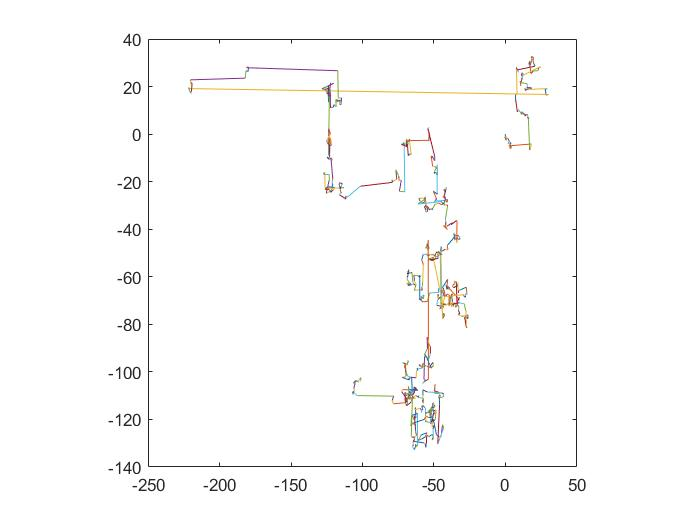
\includegraphics[width=8cm]{figure/13.jpg}\\
		\caption{Levy分布轨迹图}\label{fig13}
	\end{figure}
	
}

\frame{\frametitle{莱维过程}
	\parindent=19pt	
	\renewcommand{\raggedright}{\leftskip=0pt \rightskip=0pt plus 0cm}
	\raggedright	
	莱维过程$\{X(t),t\ge0\}$是一种随机过程,它满足的条件比布朗运动宽松:
	
	1.$X(0)$ 几乎处处为0;
	
	2.独立增量性;
	
	3.稳定增量性;
	
	4.样本轨道右连续。
	
	连续的布朗运动和离散的泊松过程都是莱维过程的特例。因此可以大胆猜测,莱维过程就是带“跳跃”的布朗运动。正是这些不连续性 的“跳跃”给予莱维过程“重尾”的特性。
}

\frame{\frametitle{莱维过程}
	\parindent=19pt	
	\renewcommand{\raggedright}{\leftskip=0pt \rightskip=0pt plus 0cm}
	\raggedright	
	\textbf{独立增量:}
	
	设$X(t)$是一个连续时间上的随机过程。也就是说,对于任何固定的$t\ge0$,$X(t)$是一个随机变量。过程的增量为差值$X(s)-X(t)$。独立增量意味着对于任意时间$s>t>u>v,X(s)-X(t)$与$X(u)-X(v)$相互独立。
	
	\textbf{稳定增量:}
	
	如果增量$X(s)-X(t)$的分布只依赖于时间间隔$s-t$,则称增量是稳定的。例如对于维纳过程,增量$X(s)-X(t)$服从均值为0,方差为$s-t$的正态分布。对于泊松过程,增量$X(s)-X(t)$服从指数为$s-t$的泊松分布。
}

\frame{\frametitle{莱维过程}
	\parindent=19pt	
	\renewcommand{\raggedright}{\leftskip=0pt \rightskip=0pt plus 0cm}
	\raggedright	
	\textbf{定理1}(莱维-辛钦公式):
	莱维过程$\{X(t),t\ge0\}$的特征函数(傅里叶变换)表达如下:
	\begin{equation}
	\phi_X(\theta)(t):=E[e^{i\theta X(t)}]=\exp(t(ai\theta-\frac{1}{2}\sigma^2\theta^2+\int_{\mathcal{R} \backslash \{0\}}(e^{i\theta x}-1-i\theta xI_{|x|<1})\prod(dx))).
	\end{equation}
	这个定理的证明比较复杂,依赖于测度论中的一系列结果。
}
\frame{\frametitle{莱维过程}
	\parindent=19pt	
	\renewcommand{\raggedright}{\leftskip=0pt \rightskip=0pt plus 0cm}
	\raggedright	
	\textbf{定理2}(莱维-伊藤分解):
	每个莱维过程$\{X(t),t\ge0\}$都可以分解为$\{S(t),t\ge0\}$,$\{Y(t),t\ge0\}$ 和$\{Z(t),t\ge0\}$三个子过程,其中:
	
	1.$S(t)$ 是维纳过程(就是布朗运动,莱维过程的连续部分);
	
	2.$Y(t)$ 是复合泊松过程(刻画了较极端的“跳跃”现象);
	
	3.$Z(t)$ 是平方可积的离散鞅(刻画了较小的“跳跃”现象)。
}

\frame{\frametitle{Basic Definition}
	\parindent=19pt	
	\renewcommand{\raggedright}{\leftskip=0pt \rightskip=0pt plus 0cm}
	\raggedright	
	随机变量(r.v.)$X\sim\mu$的特征函数是映射$\Phi:\mathbf{R}^d\to\mathbb{C}$,定义如下
	\begin{equation}
	\Phi(u)=\mathbb{E}(e^{iu\cdot X})=\int_{R^d}e^{iu\cdot y}\mu(dy).
	\end{equation}
	随机变量$X$是无限可分的,除非它的该率分布$p_x$是无限可分的,例如,$X=Y_1^{(n)}+...+Y_n^{(n)}$,其中$Y_1^{(n)},...,Y_n^{(n)}$是独立同分布。那么$X$的特征函数可以写成$\Phi_X(u)=(\Phi_{Y_1^{(n)}}(u))^n$.
	
	\textbf{定义1:}
	
	莱维可测是满足如下条件的$\mathbb{R}^d\backslash\{0\}$上的测度$v$,使得
	\begin{equation}
	\int(|y|^2\wedge1)v(dy)<\infty.
	\end{equation}
	其中$|y|^2\wedge1=\left\{\begin{array}{cc}1,&|x|>1\\
	y^2,&|x|\le1\end{array}\right.$
}

\frame{\frametitle{Levy-Ito decomposition}
	\parindent=19pt	
	\renewcommand{\raggedright}{\leftskip=0pt \rightskip=0pt plus 0cm}
	\raggedright	
	定义函数$X:\mathbf{R}^{+}\to\mathbf{R}$是Cadlag过程,即$X$是右连续左极限存在。令$\Delta X(t)=X(t)-X(t-)$(由于左极限的存在)且定义如下泊松随机测度
	\begin{equation}
	N(t,A)=\sharp \{\Delta X(s)\in A:s\in[0,t]\}.
	\end{equation}
	那么有如下结论:
	
	(1)$N(1,B_{\varepsilon}^c(0))<\infty$.
	
	(2)$N(1,\mathbf{R}\backslash \{0\})$是可数的。
	
	令$A$是有下界的,i.e., $0\not\in\overline{A}$.那么$N(t,A),t\ge0$是泊松过程且强度为$\mu(A)=\mathbf{E}[N(1,A)]$.很明显有结论$\mu(A)<\infty$不管$A$ 是否有下界。所以测度$\mu$是$\sigma-$有限的。
}
\frame{\frametitle{Levy-Ito decomposition}
	\parindent=19pt	
	\renewcommand{\raggedright}{\leftskip=0pt \rightskip=0pt plus 0cm}
	\raggedright	
	\textbf{推论1:}
	(1)对任意的$t>0,\omega\in\Omega,N(t,\cdot)(\omega)$在$\mathcal{B}(\mathbf{R}^d\backslash \{0\})$上是计数可测的。
	
	(2)对于任意的有下界的$A$,$N(t,A),t\ge0$是泊松过程且具有如下强度$\mu(A)=\mathbf{E}[N(1,A)]$.
	
	(3)补$\tilde{N}(t,A)=N(t,A)-t\mu(A)$是值鞅可测的。对于有下界的$A$, $\tilde{N}(t,A)$是一个鞅。
	
	令$f:\mathbf{R}^d\to\mathbf{R}$是波莱尔可测函数,$A$有下界,那么对任意$t>0,\omega\in\Omega$,我们定义如下关于$f$泊松积分通过一个随机有限和。
	\begin{equation}
	\int_{A}f(x)N(t,dx)(\omega)=\sum_{x\in A}f(x)N(t,\{x\})(\omega).
	\end{equation}
}
\frame{\frametitle{Levy-Ito decomposition}
	\parindent=19pt	
	\renewcommand{\raggedright}{\leftskip=0pt \rightskip=0pt plus 0cm}
	\raggedright	
	\textbf{定理2:}令$A$有下界,则
	
	(1)对任意的$\int_{A}f(x)N(t,dx),t\ge0$是复合泊松过程,带有如下特征函数:
	\begin{equation}
	\mathbf{E}[exp\{iu\cdot\int_{A}f(x)N(t,dx)\}]=exp\{t\int_{A}(e^{iu\cdot x}-1)\mu_f(dx)\}.
	\end{equation}
	其中$u\in\mathbf{R}^d,\mu_f=\mu\circ f^{-1}$.
	
	(2)如果有$f\in L^1(A,\mu_A)$,那么有
	\begin{equation}
	\mathbf{E}[\int_{A}f(x)N(t,dx)]=t\int_{A}f(x)\mu(dx).
	\end{equation}
	
	(3)如果有$f\in L^2(A,\mu_A)$,那么有
	\begin{equation}
	Var[|\int_{A}f(x)N(t,dx)|]=t\int_{A}|f(x)|^2\mu(dx).
	\end{equation}
}

\frame{\frametitle{Levy-Ito decomposition}
	\parindent=19pt	
	\renewcommand{\raggedright}{\leftskip=0pt \rightskip=0pt plus 0cm}
	\raggedright	
	从定理2可以看出,如果$f\in L^1(A,\mu_A)$,一个泊松积分也许不一定全都有有限期望。对于此,我们定义如下补泊松积分:
	\begin{equation}
	\int_{A}f(x)\tilde{N}(t,dx)=\int_{A}f(x)N(t,dx)-t\int_{A}f(x)\mu(dx).
	\end{equation}
	则有如下结论:
	
	(1) $\int_{A}f(x)\tilde{N}(t,dx),t\ge0$是一个鞅。
	
	(2)
	特征函数:
	\begin{equation}
	\mathbf{E}[exp\{iu\cdot\int_{A}f(x)\tilde{N}(t,dx)\}]=exp\{t\int_{A}(e^{iu\cdot x}-1-iu\cdot x)\mu_f(dx)\}.
	\end{equation}
	其中$u\in\mathbf{R}^d,\mu_f=\mu\circ f^{-1}$.
	
	
	(3)如果有$f\in L^2(A,\mu_A)$,那么有
	\begin{equation}
	Var[|\int_{A}f(x)\tilde{N}(t,dx)|]=t\int_{A}|f(x)|^2\mu(dx).
	\end{equation}
}
\frame{\frametitle{Levy-Ito decomposition}
	\parindent=19pt	
	\renewcommand{\raggedright}{\leftskip=0pt \rightskip=0pt plus 0cm}
	\raggedright	
	对于有下界的$A$和任意的$t>0$,$\int_{A}xN(t,dx)\sum_{0\le u\le t}\Delta X(u)1_A(\Delta X(u))$是集合$A$中不超过时间$t$的所有跳变值和。由于轨迹$X$ 是Cadlag,所以上述是个有限随机和。特别地,$\int_{|x|\ge1}xN(t,dx)$is所有大于1的跳变之和。也就是说是一个带有有限次扰动的复合泊松过程。相反地,也可以证明$X(t)-\int_{|x|\ge1}xN(t,dx)$带有有限次有次序动作的莱维过程。但是也许有无界扰动。所以我们可以定义
	\begin{equation}
	b=\mathbf{E}[X(1)-\int_{|x|\ge1}xN(1,dx)].
	\end{equation}
	
}

\frame{\frametitle{Levy-Ito decomposition}
	\parindent=19pt	
	\renewcommand{\raggedright}{\leftskip=0pt \rightskip=0pt plus 0cm}
	\raggedright	
	现在把关注度放在小跳变上来。引入$M(t,A)=\int_{A}f(x)\tilde{N}(t,dx)$.令$A_m=\{x:\frac{1}{m+1}<|x|\le1\}$.可以证明在$L^2$里,当$m\to\infty$ 时,我们有$M(t,A_m)\to\int_{|x|<1}x\tilde{N}(t,dx)$。所以$\int_{|x|<1}x\tilde{N}(t,dx)$是一个鞅。取极限得
	\begin{equation}
	\mathbf{E}[exp\{iu\cdot\int_{A}x\tilde{N}(t,dx)\}]=exp\{t\int_{A}(e^{iu\cdot x}-1-iu\cdot x)\mu(dx)\}.
	\end{equation}
	最后考虑如下随机过程
	\begin{equation}
	W_{A}(t)=X(t)-bt-\int_{|x|<1}x\tilde{N}(t,dx)-\int_{|x|\ge1}xN(t,dx).
	\end{equation}
	那么随机过程$W_A(t)$是带有连续采样路径的中心鞅。利用布朗运动的莱维特征化,我们有$W_A(t)$就是协方差为$A$的布朗运动。
}

\frame{\frametitle{Levy-Ito decomposition}
	\parindent=19pt	
	\renewcommand{\raggedright}{\leftskip=0pt \rightskip=0pt plus 0cm}
	\raggedright	
	\textbf{Levy-Ito Decomposition}$X$是莱维过程。那么存在$b\in\mathbf{R}^d$, 协方差为$A$的布朗运动$W_A(t)$,$\mathbf{R}^{+}\times\{\mathbf{R}^d\backslash \{0\}\}$ 独立的泊松随机测度$N$使得下式成立:
	\begin{equation}
	X(t)=bt+W_{A}(t)+\int_{|x|<1}x\tilde{N}(t,dx)+\int_{|x|\ge1}xN(t,dx).
	\end{equation}
	其中平方可积鞅($L^2$-鞅)$\int_{|x|<1}x\tilde{N}(t,dx)$是所有小跳变的补和。上述跳变是以1为界的,可以推广至任意实数$R>0$,我们有
	\begin{equation}
	X(t)=b_Rt+W_{A}(t)+\int_{|x|<R}x\tilde{N}(t,dx)+\int_{|x|\ge R}xN(t,dx).
	\end{equation}
	其中$b_R=\mathbf{E}[X(1)-\int_{|x|\ge R}xN(1,dx)]$.可以计算如下:
	
	(1)如果$1<R<\infty$,有$b_R=b+\int_{1\le|x|x<R}x\mu(dx).$
	
	(2)如果$0<R<1$,有$b_R=b-\int_{R\le|x|x<1}x\mu(dx).$
}

\frame{\frametitle{Levy-Ito decomposition}
	\parindent=19pt	
	\renewcommand{\raggedright}{\leftskip=0pt \rightskip=0pt plus 0cm}
	\raggedright	
	是否可以去除上届约束$R$呢?此时我们有
	\begin{equation}
	X(t)=b_{\infty}t+W_{A}(t)+\int_{|x|\ge 0}x\tilde{N}(t,dx).
	\end{equation}
	结论是可以的,如果我们有$\mathbf{E}[X(1)]<\infty$。此时,我们有$b_{\infty}=\textbf{E}[X(1)]<\infty$.
}

%\frame{\frametitle{布朗运动}
%\parindent=19pt	
%\renewcommand{\raggedright}{\leftskip=0pt \rightskip=0pt plus 0cm}
%\raggedright	
%最初由英国生物学家布朗(Brown)于1827年提出这种物理现象。1905年爱因斯坦首次对这一现象的物理规律给出数学描述。1918年维纳(Wiener)运用数学理论严格描述这种无规则运动。并用随机过程理论和概率理论建立了数学模型。因此又称为维纳过程。是具有\textcolor{red}{连续时间参数}和\textcolor{red}{连续状态空间}的一类随机过程。
%
%\textbf{定义:}若随机过程$\{X(t),t\ge0\}$满足:
%
%(1)$X(t)$关于$t$是连续函数;且几乎 处处不可微。
%
%(2)$\{X(t),t\ge0\}$具有平稳独立增量:对任意的有限正数$0=t_0<t_1<\cdots<t_n$,随机变量$X(t_0),X(t_1)-X(t_0),...,X(t_n)-X(t_{n-1})$相互独立。
%
%(3)$\forall s,t>0,\text{ s.t. } X(s+t)-X(s)\sim N(0,\sigma^2t)$
%
%则称随机过程$\{X(t),t\ge0\}$为布朗运动(或维纳过程)。当$\sigma=1$时,称随机过程$\{X(t),t\ge0\}$为标准布朗运动。记为$\{B(t),t\ge0\}$。\textcolor{red}{几何布朗运动}是连续时间情况下的随机过程,其中随机变量的对数遵循布朗运动。其在金融学中有所应用。
%}
%
%\frame{\frametitle{布朗运动}
%\parindent=19pt	
%\renewcommand{\raggedright}{\leftskip=0pt \rightskip=0pt plus 0cm}
%\raggedright	
%布朗运动连续性如下仿真效果:
%\begin{figure}
%  \centering
%  % Requires \usepackage{graphicx}
%  \includegraphics[width=8cm]{5/figure/15.jpg}\\
%  \caption{}\label{fig15}
%\end{figure}
%
%}
%
%\frame{\frametitle{布朗运动}
%\parindent=19pt	
%\renewcommand{\raggedright}{\leftskip=0pt \rightskip=0pt plus 0cm}
%\raggedright	
%\textbf{定义:}概率空间$(\Omega,\mathcal{F},\mathbb{P})$上的随机过程$\{X(t),t\ge0\}$称为高斯过程,若对任意的$n\ge1,t_1,t+2,...,t_n,(X(t_1),...,X(t_n))$服从高斯分布。
%
%\textbf{定理:}设$B=\{B(t),t\ge0\}$是零初值的实值随机过程。则它是布朗运动的充要条件是它是一个高斯过程,并且$\mathbb{E}(B(t))=0,\mathbb{E}(B(t)B(s))=t\wedge s=\min(s,t).$
%
%\textbf{证明:}必要性。由独立增量性$n\ge1,t_1,t+2,...,t_n,(X(t_1),...,X(t_n))$服从高斯分布。又因为
%\begin{equation}
%\left(\begin{array}{c}B(t_1)\\
%                      B(t_2)\\
%                      \vdots\\
%                      B(t_n)\end{array}\right)=\left(\begin{array}{ccccc}1&0&0&\cdots&0\\
%                      1&1&0&\cdots&0\\
%                      \vdots&\vdots&\vdots&\ddots&\vdots\\
%                      1&1&1&\cdots&1\end{array}\right)\left(\begin{array}{c}B(t_1)\\
%                      B(t_2)-B(t_1)\\
%                      \vdots\\
%                      B(t_n)-B(t_{n-1})\end{array}\right)
%\end{equation}
%}
%
%\frame{\frametitle{布朗运动}
%\parindent=19pt	
%\renewcommand{\raggedright}{\leftskip=0pt \rightskip=0pt plus 0cm}
%\raggedright	
% 所以有$(B(t_1),...,B(t_n))$服从高斯分布。显然有$\mathbb{E}(B(t))=0,$对任意$t\ge s\ge0$,有
% \begin{equation}
% \mathbb{E}(B(t)B(s))=E(B(t)-B(s))B(s)+\mathbb{E}B^2(s)=s.
% \end{equation}
%
%充分性。先证独立增量性。由于它们服从正态分布,所以只需要证明不相关性即可。事实上,对任意的$i<j$,有
%\begin{equation}
%\begin{split}
%\mathbb{E}(B(t_i)-B(t_{i-1}))(B(t_j)-B(t_{j-1}))=&\mathbb{E}B(t_i)B(t_j)-\mathbb{E}B(t_{i-1})B(t_j)\\
%                                                 &+\mathbb{E}B(t_{i-1})B(t_{j-1})\\
%                                                 &=t_i-t_i-t_{i-1}+t_{i-1}=0.
%\end{split}
%\end{equation}
%显然,对任意的$t>s,B(t)-B(s)$服从正态分布,均值为0,方差为
%\begin{equation}
%\mathbb{E}(B(t)-B(s))^2=\mathbb{E}B^2(t)-2\mathbb{E}B(t)B(s)+\mathbb{E}B^2(s)=t-s.
%\end{equation}
%}
%
%\frame{\frametitle{布朗运动的构造}
%\parindent=19pt	
%\renewcommand{\raggedright}{\leftskip=0pt \rightskip=0pt plus 0cm}
%\raggedright	
%下面利用Fourier级数直接构造布朗运动。 假设$B$是一个标准布朗运动。定义过程$W(t)=B(t)-tB(1),t\in[0,1]$.称为$[0,1]$上的布朗桥。注意到$W(0)=W(1)=0$.我们将$W$在$[0,1]$上的Fourier展开($L^2$ 意义下)
% \begin{equation}
% W(t)=\sum_{n=1}^{\infty}X_nsin(n\pi t)
% \end{equation}
% 其中系数$X_n$是随机变量,表达式为
% \begin{equation}
% X_n=2\int_0^tW(t)sin(n\pi t)dt.
% \end{equation}
% 则$X_n$服从正态分布,可以计算
% \begin{equation}
% \mathbb{E}X_n=0,\mathbb{E}[X_nX_m]=\frac{2}{\pi^2n^2}\delta_{mn}.
% \end{equation}
% 令$Z_0=B_1,Z_n=n\pi X_n/\sqrt{2},n\ge1.$ 则$\{Z_n\}$ i.i.d~$N(0,1)$。我们可以将布朗运动写成
% \begin{equation}
% B(t)=tZ_0+\frac{\sqrt{2}}{\pi}\sum_{j=1}^{\infty}\frac{Z_n}{n}sin(n\pi t),t\in[0,1].
% \end{equation}
%}
%
%\frame{\frametitle{布朗运动的逼近}
%\parindent=19pt	
%\renewcommand{\raggedright}{\leftskip=0pt \rightskip=0pt plus 0cm}
%\raggedright	
%三种逼近方式:
%
%(1)基于随机游动的逼近;
%
%(2)布朗运动的帕里-维纳表示;
%
%(3)基于小波函数的逼近方法。
%}
%\frame{\frametitle{随机漫步}
%\parindent=19pt	
%\renewcommand{\raggedright}{\leftskip=0pt \rightskip=0pt plus 0cm}
%\raggedright	
%假想一个粒子在水平直线上一步步的左右移动而且每步的距离皆为一个单位长度。其向右及向左的概率各位$p$与$q=1-p(0<p<q)$。假设每一单位时间只移动一步而且在第$n$个瞬间独立做动作。其数学模型如下:
%
%设$X_n$为粒子第$n$的位移,则$X_n:\in\mathbf{N}$为一族取值为$\{+1,-1\}$的独立随机数,而且对任一整数,我们有
%\begin{equation}
%\begin{split}
%&P\{X_n=1\}=p\\
%&P\{X_n=-1\}=q
%\end{split}
%\end{equation}
%若以$W_0$表示粒子的原始位置,则在时间$n$时粒子的位置为
%\begin{equation}
%W_n=W_0+X_1+X_2+\cdots+X_n
%\end{equation}
%序列$\{W_n,n=0,1,2,...\}$便叫做随机漫步或者随机游走。$\{W_n\}$所在的样本空间$\Omega$可取为
%\begin{equation}
%\Omega=\{\omega:\omega=(\omega_0,\omega_1,...),\omega_i\in\mathbf{Z}\}.
%\end{equation}
%
%}
%
%\frame{\frametitle{随机漫步}
%\parindent=19pt	
%\renewcommand{\raggedright}{\leftskip=0pt \rightskip=0pt plus 0cm}
%\raggedright	
%令$P_n^r(i,j)=P\{W_{n+r}=j|W_n=i\},P_n(i,j)=P_n^1(i,j),p_{ij}=P_0(i,j),p_{ij}^r=P_0^r(i,j).$ 显然,当$i=j$时$p_{ij}^0=1,$ 否则$p_{ij}^0=0$.
%
%\textbf{定理:}
%1.$0\le P_n^r(i,j)\le1$,而且$\sum_{j\in\mathbf{Z}}P_n^r(i,j)=1$.
%
%2.$P\{W_{n+r}=j|W_0=i_0,...,w_n=i_n\}=P\{W_{n+r}=j|W_n=i_n\}=P_n^r(i_n,j),\forall r\ge1.$
%
%3.$P_n^r(i,j)=P_0^r(i,j)=p_{ij}^r$,特别地
%\begin{equation}
%P\{W_{n+r}=j|W_n=i\}=p_{ij}=\left\{\begin{array}{cc}p,&j=i+1\\
%                                                    q,&j=i-1\\
%                                                    0,&j=i
%                                                    \end{array}\right.
%\end{equation}
%4.设$0\le n_1<n_2<n_3<\cdots<n_k,$则$\{W_{n_k}-W_{n_{k-1}},....,W_{n_2}-W_{n_1}\}$为独立随机变量。
%}
%
%
%\frame{\frametitle{随机漫步}
%\parindent=19pt	
%\renewcommand{\raggedright}{\leftskip=0pt \rightskip=0pt plus 0cm}
%\raggedright	
%上述性质2说明当现在位置已知时,过去与未来无关。性质3表示粒子位置从$i$转移到$j$的概率与原位置时间无关,此性质叫做时间齐一性(马尔科夫性质)。则其转移矩阵记为
%\begin{figure}
%  \centering
%  % Requires \usepackage{graphicx}
%  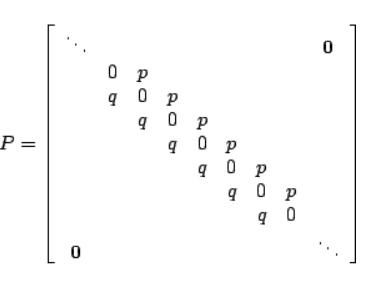
\includegraphics[width=8cm]{5/figure/16.png}\\
%  \caption{}\label{fgi16}
%\end{figure}
%
%}
%
%\frame{\frametitle{随机漫步}
%\parindent=19pt	
%\renewcommand{\raggedright}{\leftskip=0pt \rightskip=0pt plus 0cm}
%\raggedright	
%令$\mathbf{A}\subseteq\mathbf{Z}$。定义$f_{\mathbf{A}}(i)=P\{W_k\in\mathbf{A},\forall  k\ge1|W_0=i\}(i\in\mathbf{A})$。$f_{\mathbf{A}}(i)$表示$\{W_n\}$从$i$出发一直留在$\mathbf{A}$中的概率。
%
%\textbf{定理:}若$\mathbf{A}$只包含有限个整数,则$f_{\mathbf{A}}(i)=0,\forall i\in\mathbf{A}$.
%
%上述定理表明随机漫步的粒子非常不安于位。一直在做无规则运动。
%
%\textbf{定理:}$\mathbf{E}[W_{n+k}|W_n=i]=i$.(此处讨论$p=q$的性质。)
%}

%
%%%%%%
%%%%%%
%SDE 6
\section{随机微分方程}
	\frame{
	\centerline{\textbf{\Huge{随机微分方程}}}
}
 \begin{frame}

\frametitle{大纲}

\begin{itemize}
	\item 基本概念:\\
	随机过程、布朗运动、Ito积分、SDE...
	\item SDE的数值解
	\item SDE的参数估计
	
\end{itemize}



\end{frame}



\begin{frame}

\frametitle{随机过程}
\small

\textbf{例:} 我们在某一时段对某一地区成人的身高和体重(X, Y)进行随机抽样,可得出 
$$Z = (X,Y) \sim N(\mu_1,\mu_2,\rho,\sigma^2_1,\sigma^2_1)$$
$$Z(\omega) = (X(\omega),Y(\omega))$$

这是某时段所考查随机变量的概率分布,如果\textit{每隔10年}在同一地区做同样的随机抽样,得: \\
$$Z(\omega,0)=(X(\omega,0),Y(\omega,0)) \sim N(\mu_{01},\mu_{02},\rho_0,\sigma^2_{01},\sigma^2_{02})$$

第1个10年:$Z(\omega,1)=(X(\omega,1),Y(\omega,1)) \sim N(\mu_{11},\mu_{12},\rho_1,\sigma^2_{11},\sigma^2_{12})$

第2个10年:$Z(\omega,2)=(X(\omega,2),Y(\omega,2)) \sim N(\mu_{21},\mu_{22},\rho_2,\sigma^2_{21},\sigma^2_{22})$

......

第t个10年:$Z(\omega,t)=(X(\omega,t),Y(\omega,t)) \sim N(\mu_{t1},\mu_{t2},\rho_t,\sigma^2_{t1},\sigma^2_{t2})$ $t = 0,1,2...$

因此$\{Z(\omega,t)=(X(t),Y(t)): t \geq 0\}$表示的就是身高和体重这两个随机变量在不同时段的情况。


\end{frame}


\begin{frame}

\frametitle{随机过程}

\begin{definition}[随机过程]

设 $(\Omega ,{\mathcal  {F}},P)$为一概率空间,另设集合T为一指标集合,如果对于所有$t\in T$,均有一随机变量 $X(t,\omega)$定义于概率空间$(\Omega ,{\mathcal  {F}},P)$,则集合$\{X(t,\omega)|t\in T\}$为一随机过程

\begin{itemize}

\item 对于固定的$\omega$, 比如$\overline{\omega}$, $\{X(t,\overline{\omega}), t \geq 0\}$被称为\textbf{路径(path)}或\textbf{轨迹(trajectory)}

\item 对于固定的t,比如$\overline{t}$,集合$\{X(\overline{t},\omega), \omega \in \Omega\}$是时刻$\overline{t}$在该随机过程中的状态集,$X(\overline{t},\omega)$也就是时刻$\overline{t}$的随机变量


\end{itemize}

\end{definition}

\end{frame}

\begin{frame}

\frametitle{布朗运动}	

\begin{proof}

设连续时间随机过程$W_t: 0 \leq t < T$ 是 $[0,T)$上的标准布朗运动,

\begin{itemize}

\item $W_0 = 0$

\item \textbf{独立增量性:} 对于有限个时刻$0 \leq t_1 < t_2 < ... < t_n < T$,随机变量$$W_{t_2}-W_{t_1},W_{t_3}-W_{t_2},...,W_{t_n}-W_{t_{n-1}}$$是独立的

\item \textbf{正态性:} 对任意的$0 \leq s < t < T$, $W_t-W_s$服从均值为0,方差为t-s的正态分布

\end{itemize}

\end{proof}

\end{frame}

\begin{frame}

\frametitle{随机微分方程}

一般的随机微分方程$$\frac{\mathrm{d}X(t)}{\mathrm{d}t}=h[X(t),t]+g[X(t),t]R(t)$$
形式上$$R(t)=\frac{\mathrm{d}B}{\mathrm{d}t}$$
其中记号$\mathrm{d}W(t)=R(t)\mathrm{d}t$,$B(\omega,t)$是维纳过程 \\
对上式求积分,得:$$X(t)-X(0)=\int_0^t h[s,X(s)]\mathrm{d}s + \int_0^t g[s,X(s)]\mathrm{d}B$$
第一个积分是普通微积分的,第二个积分是维纳过程的随机函数的积分\\
布朗运动:$\mathrm{d}X_t = \mu \mathrm{d}t + \sigma\mathrm{d}W_t$\\
几何布朗运动:$\mathrm{d}X_t = \mu X_t\mathrm{d}t + \sigma X_t\mathrm{d}W_t$

\end{frame}

\begin{frame}

\frametitle{随机积分的求解}
\footnotesize  

与普通微积分的牛顿莱布尼茨公式采用分区间近似求和相同,随机微积分中也是用分片的常数函数来近似$g[s,X(s)]$,即$$\int_0^tg[s,X(s)]\mathrm{d}B \approx \sum_{i=0}^{n-1}g_i[s,X(s)]\mathrm{d}B_i = \sum_{i=0}^{n-1}g_i[s,X(s)][B(t_{i+1})-B(t_i)], s \in [t_{i+1},t_i]$$
其中s的取值有两种:

\begin{itemize}

\item 在区间左端点$t_i$取值$$g_i[s,X(s)]=G[t_i,X(t_i)]$$
相应的随机积分$$\int_0^t g[s,X(s,\omega)]\mathrm{d}B(\omega,t)$$
称为Ito积分

\item 在区间端点取值求平均$$g_i[s,X(s)]=\frac{g[t_i,X(t_i)]+g[t_{i+1},X(t_{i+1})]}{2}$$
相应的随机积分$$\int_0^t g[s,X(\omega,s)]∘\mathrm{d}B(\omega,t)$$
称为Stratonovich积分

\end{itemize}

\end{frame}

\begin{frame}

\frametitle{随机积分的求解:例}
\footnotesize
设$g[t,B(t)]=B(t)$,则在Ito积分中:
\begin{align}
I_1 &= \int_0^t B(s)\mathrm{d}B \\ 
&\approx -\sum_{i=0}^{n-1}B_i(B_i-B_{i+1}) \\
&=-[B_0^2-B_0B_1+B_0^2-B_0B_1+...+B_{n-1}^2-B_{n-1}B_n] \\
&=-\frac{1}{2}[B_0^2+\sum_{i=1}^{n-1}(B_{i+1}-B_i)^2-B_n^2]=\frac{1}{2}(B_t^2-B_0^2)-\frac{1}{2}\sum_{i=1}^{n-1}\Delta B_i^2
\end{align}

在Stratonovich积分中:
\begin{align}
I_2 &= \int_0^t B(s)∘\mathrm{d}B \approx \sum_{i=0}{n-1}\frac{1}{2}[B(t_{i+1})+B(t_i)][B(t_{i+1})-B(t_i)]\\
&= \frac{1}{2}\sum_{i=0}{n-1}[B^2(t_{i+1})-B^2(t_i)]\\
&= \frac{1}{2}[B^2(t_1)-B^2(t_0)+B^2(t_2)-B^2(t_1)+...+B^2(t_n)-B^2(t_{n-1})]\\
&= \frac{1}{2}[B^2(t_n)-B^2(t_0)] = \frac{1}{2}B^2(t)
\end{align}

\end{frame}

\begin{frame}

\frametitle{Ito公式}
\footnotesize

普通微积分中,若X连续可微,则$$X(t)-X(0)=\sum_{i=1}^n[X(t_i)-X(t_{i-1})]=\sum_{i=1}^nX'({\xi}_i)(t_i-t_{i-1})=\int_0^t X'(s)\mathrm{d}s$$

将t替换成$B_t$,此时$\xi_i$是介于$B_{i-1}$和$B_i$之间的点,$\xi_i$在区间不同位置的取值会影响积分值,Ito将取${\xi_i}$为左端点进行求和,这就需要将泰勒公式多展开一阶
$X(B_{t_j})-X(B_{t_{j-1}}) = X'(B_{t_{j-1}})(B_{t_j}-B_{t_{j-1}})+\frac{1}{2}X''(\xi_j)(B_{t_j}-B_{t_{j-1}})^2$\\
右端第一项求和,得$$\sum_{j=1}^nX'(B_{t_{j-1}})(B_{t_j}-B_{t_{j-1}}) \rightarrow \int_0^tX'(B_s)\mathrm{d}B_s$$\\
右端第二项求和,$$\sum_{j=1}^n\frac{1}{2}X''(\xi_j)(B_{t_j}-B_{t_{j-1}})^2 \rightarrow \frac{1}{2}\int_0^tX''(B_s)\mathrm{d}s$$\\
即 $X(B_t) = X(B_0) + \int_0^tX'(B_s)\mathrm{d}B_s + \frac{1}{2}\int_0^tX''(B_s)\mathrm{d}s$\\
微分形式:$\mathrm{d}X(B_t) = X'(B_t)\mathrm{d}B_t + \frac{1}{2}F''(B_t)\mathrm{d}t$

\end{frame}

\begin{frame}
\frametitle{Ito公式的应用}
\footnotesize
假设X(t)满足几何布朗运动的SDE:$$\mathrm{d}X_t = \mu X_t\mathrm{d}t + \sigma X_t\mathrm{d}W_t$$
如何解出X(t)?\\
设$Y(t) = lnX(t)$,则$\frac{\partial Y}{\partial X} = \frac{1}{X}$,$\frac{\partial^2Y}{\partial X^2} = -\frac{1}{X^2}$,由Ito公式得:
\begin{align}
\mathrm{d}Y &= \frac{\partial Y}{\partial X}\mathrm{d}X + \frac{1}{2}\frac{\partial^2Y}{\partial X^2}(\mathrm X_t)^2\\
&= \frac{1}{X}(\mu X\mathrm{d}W) + \frac{1}{2}(-\frac{1}{X^2})\sigma^2X^2\mathrm{d}t\\
&= \mu \mathrm{d}t + \sigma \mathrm{d}W - \frac{1}{2}\sigma^2\mathrm{d}t\\
&= (\mu-\frac{1}{2}\sigma^2)\mathrm{d}t + \sigma\mathrm{d}W\\
\end{align}


\end{frame}

\begin{frame}
\frametitle{Ito公式的应用}
\footnotesize
则Y(t)是布朗运动,因此
\begin{align}
Y(t) &= Y(t_0)+(\mu-\frac{1}{2}\sigma^2)(t-t_0) + \sigma(W(t)-W{t_0})\\
X(t) &= exp(Y(t))\\
&= X(t_0)exp[(\mu-\frac{1}{2}\sigma^2)(t-t_0)+\sigma(W(t)-W(t_0))]
\end{align}

\end{frame}

\begin{frame}

\frametitle{SDE的数值解}
\footnotesize

并不是所有的SDE都能解出显式解,更多的SDE只能通过迭代式求数值解,求SDE数值解的过程也就是模拟出解的路径。
\renewcommand{\proofname}{Euler格式}
\begin{proof}
$$X_{i+1} = X_i + \mu (t_i,X_i)(t_{i+1-t_i}) + \sigma(t_i,X_i)(W_{i+1}-W_i)$$
\end{proof}

\renewcommand{\proofname}{Milstein格式}
\begin{proof}
\begin{align}
X_{i+1} &= X_i + \mu (t_i,X_i)(t_{i+1}-t_i)+\sigma (t_i,X_i)(W_{i+1}-W_i)\\
&\frac{1}{2}\sigma(t_i,X_i)\sigma_y(t_i,X_i)\{(W_{i+1}-W_i)^2-(t_{i+1}-t_i)\}
\end{align}

\end{proof}

其中$$W_{i+1}-W_i = \sqrt{t_{i+1}-t_i}Z_{i+1}, i=0,1,...,n-1$$
而$Z_1,...,Z_n$是相互独立的标准正态随机变量

\end{frame}

\begin{frame}

\frametitle{SDE的参数估计}
\begin{itemize}
\item 极大似然估计
\end{itemize}
以布朗运动$\mathrm{d}X_t = \mu(X_t;\theta)\mathrm{d}t + \sigma(X_t;\theta)\mathrm{d}W_t$为例
假设$x_0,...,x_N$是$X(t)$在均匀离散时刻$t_i = \Delta t$的观测,其中$i = 0,1,...,N, \Delta t = T/N.$\\
令$p(t_k,x_k|t_{k-1},x_{k-1;\theta})$是从$(t_{k-1},x{k-1})$到$(t_k,x_k)$的传递概率密度,\\
假设初始状态的概率密度为$p_0(_0|\theta)$,似然函数为:$$f(\theta) = p_0(x_0|\theta)\prod_{k=1}^Np(t_k,x_k|t_{k-1},x_{k-1};\theta)$$
考虑SDE的Euler近似,有$$X(t_k) = x_{k-1} + \mu (t_{k-1},x_{k-1};\theta)\Delta t + \sigma(t_{k-1},x_{k-1};\theta)\sqrt{\Delta t}\eta_k$$
其中$\eta_k \sim N(0,1)$。因此
$$p(t_k,x_k|t_{k-1},x_{k-1};\theta) = \frac{1}{\sqrt{2\pi\sigma_k}}exp(-\frac{(x_k-\mu_k)^2}{2\sigma_k^2})$$
其中$\mu_k = x_{k-1} + \mu(t_{k-1},x_{k-1};\theta), \sigma_k = \sigma(t_{k-1},x_{k-1};\theta)\sqrt{\Delta t}$

\end{frame}

\begin{frame}

\frametitle{SDE的参数估计}
\begin{itemize}
\item 实例:种群动力学
\end{itemize}

考虑美洲鹤1939-1985年的种群数据,假设t时刻种群大小X(t)满足SDE:$$\mathrm{d}X(t) = \theta_1X(t)\mathrm{d}t + \theta_2\sqrt{X(t)}\mathrm{d}W(t), X(0) = 18$$

\begin{center}
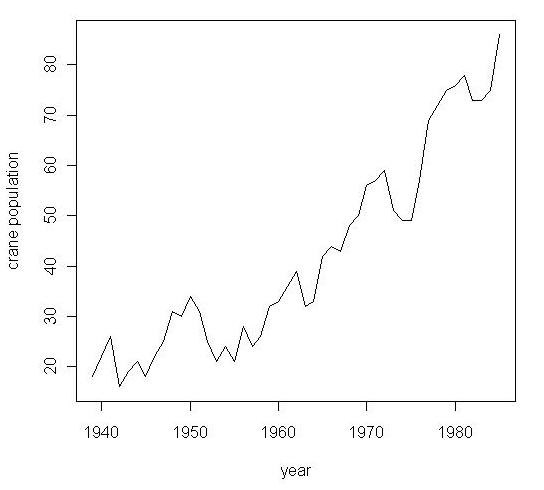
\includegraphics[width = .6\textwidth]{goose.png}
\end{center}

\end{frame}

%
%%%
%application final
\section{觅食算法实例}
\frame{
	\centerline{\textbf{\Huge{觅食算法实例}}}
}
\begin{frame}
\frametitle{概览}
%\framesubtitle{}
\begin{itemize}
\item 资源分配和调度
\item 信号处理
\item 预测控制
\item 图形图像
\end{itemize}
\end{frame}

\begin{frame}
%\frametitle{觅食算法实例}
\frametitle{资源分配和调度}
\begin{itemize}
\item 对计算机中的多区域温度调度平台(\textit{Multizone Temperature Experimentation Platform})进行资源分配,以低温区域为“食物”,细菌的觅食过程就是将数据的获取与计算工作分配至低温区域以获得更高的能效
\item 车间作业中利用觅食算法进行空闲时间片段的调度,将未完成的工序合理地分配到不同的空闲时间中。在工序顺序和机器占用的约束下,有效降低调度的规模和复杂性
\end{itemize}
\end{frame}

\begin{frame}
%\frametitle{觅食算法实例}
\frametitle{信号处理}
独立组分分析(ICA)用来对统计信号进行处理,找到非高斯分布数据的线性表示。利用觅食算法与ICA的结合,可以提高信号处理的收敛速度,降低均方误差
\end{frame}

\begin{frame}
%\frametitle{觅食算法实例}
\frametitle{预测控制}
\begin{itemize}
\item 利用觅食算法对股票市场指数趋势进行预测
\item 利用觅食算法对控制系统进行局部优化
\end{itemize}
\end{frame}

\begin{frame}
%\frametitle{觅食算法实例}
\frametitle{图形图像}
利用细菌觅食算法,在图像识别中,提高识别的速度与准确率。通常会与基因算法等其他算法进行结合,在面部识别等领域提高特征点的搜索速度。
\end{frame}

\end{document}